\documentclass{article}

\PassOptionsToPackage{numbers, compress}{natbib}
\usepackage[preprint]{neurips_2026}

\usepackage[utf8]{inputenc}
\usepackage[T1]{fontenc}
\usepackage{hyperref}
\usepackage{url}
\usepackage{booktabs}
\usepackage{amsfonts}
\usepackage{amsmath}
\usepackage{amssymb}
\usepackage{nicefrac}
\usepackage{microtype}
\usepackage{xcolor}
\usepackage{graphicx}
\usepackage{subcaption}
\usepackage{multirow}
\usepackage{float}

\graphicspath{{figures/}}

\title{Emotion-Informed MBTI Prediction}

\author{%
  Harry Hu \quad Tom Shan \quad Wendy Wang \quad Kemeng Zhang \\
  Group 66 \\
  AC~209b / CS~1090b, Spring 2026 \\
  Harvard University
}

\begin{document}

\maketitle

\begin{abstract}
Automated Myers--Briggs Type Indicator (MBTI) inference from public writing is increasingly used in HR analytics, recommendation, and adaptive-learning systems despite well-documented psychometric concerns. We propose MBTI prediction from Reddit posts as an author-level task with four binary dimensions ($E/I$, $N/S$, $F/T$, $J/P$). Posts ($n{=}1.65\text{M}$) are masked for type-leakage, split by author, and aggregated into one prediction per user ($N{=}10{,}414$). We compare a TF--IDF logistic baseline and corrected text-only and text$+$emotion GRUs against frozen MiniLM author probes and a permutation-invariant \emph{set-attention} author transformer. Set-attention with a $p{=}200$ post budget gives the strongest robust mean test balanced accuracy ($0.6784$), $+0.027$ over TF--IDF and $+0.082$ over the corrected GRU (paired bootstrap, $95\%$ CI excludes zero). Adding text-derived emotion probabilities does \emph{not} robustly improve text-only performance ($\Delta{=}{-}0.007$, CI~$[-0.019,+0.004]$), and a shuffled-emotion negative control matches real emotion. We conclude that author-level set-attention is the right modeling layer, while transferred emotion features are informative but not robustly incremental.
\end{abstract}

\section{Background and motivation}

Personality has measurable correlates in language~\citep{pennebaker1999linguistic,mairesse2007using,park2015automatic}, and the MBTI taxonomy is widely used in HR analytics, recommendation, and educational platforms despite well-documented psychometric critiques~\citep{pittenger1993utility}. Two practical consequences follow: (i) automated MBTI inference is already commercially deployed, so it is worth understanding what such systems \emph{can} and \emph{cannot} learn from writing alone; and (ii) any quantitative claim should be honest about how much of the signal is text content versus correlated surface features (verbosity, vocabulary, emotion proxies).

Existing public work on Reddit MBTI prediction~\citep{plank2015personality,gjurkovic2018reddit} typically trains and evaluates on individual posts. This is a methodological problem because MBTI labels are \emph{self-reported per user}: every post by a given author inherits the same noisy label, so a post-level random split lets the model memorize the author-specific writing style that does not generalize to new users. Our project re-frames it to an author level prediction task.

\section{Problem statement}

\textbf{Research question.} Do text plus transferred emotion-informed features improve author-level prediction of the four binary MBTI dimensions over text-only baselines?

\textbf{Unit of observation.} The author. Each user $u$ has a multi-set of posts $\mathcal{P}_u = \{p_{u,1}, \ldots, p_{u,n_u}\}$ and a single self-reported MBTI label, since types are reported per-user and posts only inherit them. Training, validation, test splits are therefore stratified \emph{by author}, never by post.

\textbf{Target / output.} The MBTI label is decomposed into a four-vector $\mathbf{y}_u \in \{0,1\}^{4}$ over the dichotomies $(E/I,\,N/S,\,F/T,\,J/P)$, with the positive class chosen as the expected \emph{minority} side on Reddit: $\mathbf{y}_u = (\mathbb{1}[E],\mathbb{1}[S],\mathbb{1}[T],\mathbb{1}[J])$. The model output is a continuous score vector $\hat{\mathbf{y}}_u \in [0,1]^{4}$ at the author level, converted to a hard prediction $\tilde{\mathbf{y}}_u \in \{0,1\}^{4}$ via per-dimension thresholds $\tau_k^{*}$ tuned on validation. We do \emph{not} predict the 16-way type directly: the four binary outputs are reported and evaluated independently, which is robust to the long tail of rare types and matches downstream decisions that target one dichotomy at a time.

\textbf{Primary metric.} Mean test \emph{balanced accuracy} across the four dimensions ($\tfrac12(\mathrm{TPR}+\mathrm{TNR})$), with F1, ROC--AUC, average precision, and minority precision/recall reported. Balanced accuracy is the headline metric because three of four dimensions are strongly minority-imbalanced (Sec.~\ref{sec:data}). We declare a model strictly stronger than another only when paired bootstrap differences over test authors exclude zero at $95\%$.

\section{Data and EDA}\label{sec:data}

We use two public datasets. The Reddit MBTI corpus~\citep{kaggle_reddit_mbti} provides $13{,}028{,}455$ posts from $11{,}773$ authors with self-reported types. The \texttt{AdamCodd/emotion-balanced} corpus~\citep{hf_emotion_balanced} provides $\approx{20}\text{k}$ short texts balanced across six emotions (sadness, joy, love, anger, fear, surprise) and serves as \emph{source} supervision for emotion features that are then transferred to Reddit.

\paragraph{Preprocessing.} After EDA we adopt: (i) word-count filter ($\geq 5$ words per post), (ii) author-activity floor ($\geq 20$ posts per author), and (iii) per-author cap of $200$ posts. We also \emph{mask} explicit MBTI strings (\texttt{INTJ}, \texttt{Myers--Briggs}, etc.) with a sentinel token before any modelling: $1.66\%$ of posts and $78.4\%$ of authors mention some MBTI term, and $0.86\%$ of posts mention the author's own type (Table~\ref{tab:leakage}). Masking drives all tracked leakage counts to zero and prevents trivial token-level shortcuts. The post-budget is enforced by a deterministic per-author hash of stable row identifiers, not by chronology, because the Reddit dump does not provide reliable timestamps. After filtering, modelling uses $1{,}649{,}102$ posts from $10{,}414$ authors, split by \emph{author} into 70/15/15 ($N_{\text{train}}{=}7289$, $N_{\text{val}}{=}1562$, $N_{\text{test}}{=}1563$), stratified by MBTI type.

\begin{table}[t]
  \small
  \centering
  \caption{MBTI label-leakage audit before and after masking type tokens. Masking eliminates explicit type mentions while leaving the rest of the post intact.}
  \label{tab:leakage}
  \begin{tabular}{lrrr}
    \toprule
    Stage & Posts with any MBTI term & Authors with any term & Posts mentioning own type \\
    \midrule
    Before masking & $216{,}846$ ($1.66\%$) & $9{,}232$ ($78.4\%$) & $112{,}294$ ($0.86\%$) \\
    After masking  & $0$                    & $0$                  & $0$                    \\
    \bottomrule
  \end{tabular}
\end{table}

\paragraph{Class imbalance.} The four dichotomies are asymmetric. Test positive shares are $E{:}21.4\%$, $S{:}6.7\%$, $T{:}39.7\%$, $J{:}39.7\%$. $N/S$ in particular forces a balanced-accuracy-vs-F1 trade-off that we resolve by validation-tuned thresholds (see Methods).

\paragraph{Token length and emotion transfer.} Median post length is $22$ tokens; the $99$th percentile is $295$. A 256-token cap leaves $1.5\%$ of posts truncated and is what we use for the frozen MiniLM encoder; a 128-token cap (used by the GRU baseline) truncates $6.4\%$ (Appx.~Fig.~\ref{fig:tokenlen}). Emotion probabilities transferred onto Reddit are far from uniform: joy and anger dominate. It is consistent with social-media tone and which is why we treat them as \emph{transferred} text-derived features, not as independent measurements of a user's emotional state (Appx.~Fig.~\ref{fig:emotiondist}).

\section{Methods and models}\label{sec:methods}

\subsection{Notation}
For author $u$ with retained posts $\mathcal{P}_u$, let $\mathbf{x}_{u,i} \in \mathbb{R}^d$ be the representation of post $i$. The four-dimensional logit vector is $\boldsymbol{\ell}_u \in \mathbb{R}^4$, the post score is $\boldsymbol{\ell}_{u,i}$, and the author probability is $\hat{\mathbf{y}}_u = \sigma(\boldsymbol{\ell}_u)$. We use class-weighted binary cross-entropy
\begin{equation}
  \mathcal{L}(\boldsymbol{\ell}, \mathbf{y}) = -\sum_{k=1}^{4} \Big[ w_{k}^{+}\,y_k\log\sigma(\ell_k) + w_{k}^{-}(1-y_k)\log\big(1-\sigma(\ell_k)\big) \Big],
\end{equation}
with per-dimension weights $w_{k}^{\pm}$ derived from training prevalence using a \emph{square-root inverse-frequency} schedule, which we found to be a better trade-off than raw inverse-frequency (the latter over-shoots minority recall and collapses precision).

\subsection{Baseline layer}
\textbf{Majority.} Predict the train-set majority class for every author; pinned at balanced accuracy $0.50$ by construction.

\textbf{TF--IDF logistic.} Author documents are formed by concatenating an author's masked posts; we fit a $5000$-feature unigram+bigram TF--IDF and one balanced-class logistic regression per dimension. This is a strong content-only baseline.

\textbf{Corrected GRU (text and text$+$emotion).} The MS3 baseline collapsed to majority on three of four dimensions. We \emph{corrected} it by switching the post-level loss to class-weighted BCE, aggregating post probabilities to author-level by mean, and tuning a per-dimension decision threshold on validation:
\begin{equation}
  \hat{y}_{u,k} = \mathbb{1}\!\left[\frac{1}{|\mathcal{P}_u|}\sum_{i\in\mathcal{P}_u} \sigma\big(\ell_{u,i,k}\big) \geq \tau_k^{*}\right],\qquad
  \tau_k^{*} = \arg\max_{\tau \in [0.05,0.95]} \mathrm{BA}\big(\mathbf{y}^{\text{val}}_{k}, \mathbb{1}[\cdot \geq \tau]\big).
\end{equation}
The text-only and text$+$emotion variants share the same architecture; the latter concatenates the six emotion probabilities to the GRU pooled state before the head.

\subsection{Transferred emotion features}
A DistilBERT-class emotion classifier trained on \texttt{emotion-balanced} produces per-post probability vectors $\mathbf{e}_{u,i}\in\Delta^{5}$ over the six emotions. We treat $\mathbf{e}$ as a \emph{transferred text-derived representation}, not as a measurement of $u$'s mood: it is a deterministic function of the same words that the text encoder also sees. This framing is what motivates our negative controls below.

\subsection{Frozen transformer author probes}
We embed each post with frozen \texttt{all-MiniLM-L6-v2}~\citep{wang2020minilm,reimers2019sentencebert} into $\mathbf{x}_{u,i}\in\mathbb{R}^{384}$ and form author features by post-wise mean and standard deviation,
\begin{equation}
  \boldsymbol{\mu}_u = \frac{1}{|\mathcal{P}_u|}\sum_{i} \mathbf{x}_{u,i},\qquad
  \boldsymbol{\sigma}_u = \mathrm{std}_{i}\,\mathbf{x}_{u,i},
\end{equation}
optionally concatenated with average emotion probabilities $\bar{\mathbf{e}}_u$ and six length/activity \emph{controls} (post count, mean/median/$p90$ token count, truncation share). A logistic head is then trained per dimension. This isolates the question ``how far does a fixed transformer encoder already take us under simple pooling?'' from architectural choices.

\subsection{Set-attention author transformer (AC~209b method)}
An author is a permutation-invariant set of posts, so we use a single-block multi-head self-attention pooler with no positional encoding, in the spirit of DeepSets~\citep{zaheer2017deepsets} and Set Transformer~\citep{lee2019settransformer}. Given $\mathbf{X}_u \in \mathbb{R}^{|\mathcal{P}_u|\times d}$ (with padding to a fixed budget $P$ and a Boolean mask $m_u$):
\begin{align}
  \mathbf{H}_u &= \mathbf{X}_u \mathbf{W}_{\text{in}} \in \mathbb{R}^{P\times d_{\text{model}}}, \\
  \widetilde{\mathbf{H}}_u &= \mathrm{LN}\!\Big(\mathbf{H}_u + \mathrm{Dropout}\big(\mathrm{MHA}(\mathbf{H}_u,\mathbf{H}_u,\mathbf{H}_u;\, m_u)\big)\Big), \\
  \mathbf{z}_u &= \frac{\sum_{i} m_{u,i}\,\widetilde{\mathbf{H}}_{u,i}}{\sum_i m_{u,i}}, \qquad
  \boldsymbol{\ell}_u = \mathrm{MLP}(\mathbf{z}_u).
\end{align}
Multi-head attention (4 heads, $d_{\text{model}}{=}128$, dropout $0.2$) is permutation-equivariant; masked mean-pooling makes the author representation permutation-invariant, which is correct because Reddit chronology is unreliable.

\textbf{Variants.} Set-attention runs include \emph{text-only}; \emph{text + real emotion}, where post features are augmented with $\mathbf{e}_{u,i}$ before $\mathbf{W}_{\text{in}}$; \emph{text + shuffled emotion}, where $\mathbf{e}$ is shuffled \emph{within split} so author-emotion alignment is broken but the marginal emotion distribution is unchanged; \emph{text + controls} (length/activity controls appended at the author level); and a full \emph{text + real emotion + controls} run. Post budgets $P\!\in\!\{50,200\}$ are tested. We also compare against simple mean- and mean+std-pooled MLPs.

\subsection{Training and evaluation protocol}
All trainable models are optimised with AdamW (lr~$10^{-3}$, weight decay~$10^{-2}$) using class-weighted BCE and early stopping on validation loss. Set-attention runs use $5$ epochs by default; we additionally verify $10$/$20$ epoch caps and three random seeds (Appx.~Fig.~\ref{fig:seed}, \ref{fig:epoch}). Author-level metrics use thresholds tuned to maximise validation balanced accuracy. Confidence intervals come from \emph{paired bootstrap} over the $1{,}563$ test authors with $B{=}2000$ resamples; the per-author pairing prevents the bootstrap from confounding sampling noise with model differences. For the emotion question we adopt two estimands:
\begin{equation}
  \Delta_{\text{real}} = \mathrm{BA}_{\text{text}+\text{real emotion}} - \mathrm{BA}_{\text{text}},\qquad
  \Delta_{\text{shuf}} = \mathrm{BA}_{\text{text}+\text{shuffled emotion}} - \mathrm{BA}_{\text{text}}.
\end{equation}
If $\Delta_{\text{shuf}}$ matches or exceeds $\Delta_{\text{real}}$, the ``emotion adds signal'' claim is not supported.

\section{Results and interpretation}\label{sec:results}

\subsection{Headline comparison}

\begin{figure}[t]
  \centering
  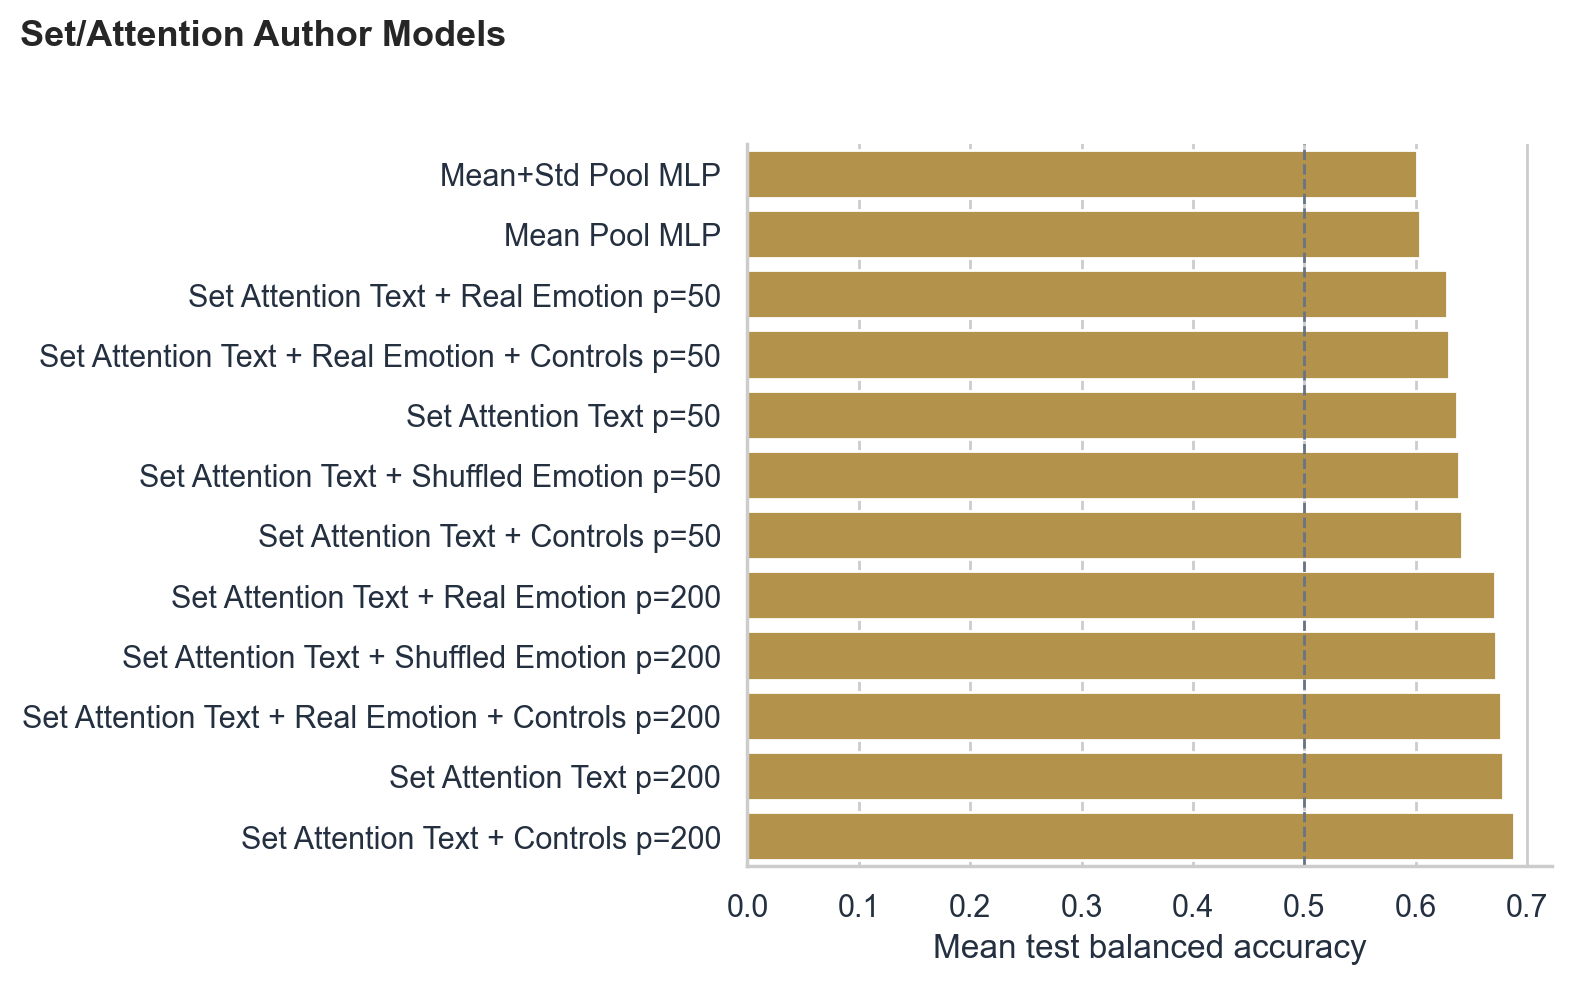
\includegraphics[width=0.85\linewidth]{fig_set_attention_author_models.png}
  \caption{Mean test balanced accuracy across set-attention author-model variants and mean-pooled MLP baselines. Set-attention at $P{=}200$ on text alone (our clean main model) reaches $0.678$; the ``$+$ Controls'' diagnostic run reaches $0.688$ but bundles activity/length features and is not promoted to the headline.}
  \label{fig:summary}
\end{figure}

Figure~\ref{fig:summary} and Table~\ref{tab:main} summarise mean test balanced accuracy across families. Set-attention at $P{=}200$ on text alone reaches $0.6784$, which is a $+0.027$ improvement over the strong TF--IDF logistic baseline ($0.6512$) and a $+0.082$ improvement over the corrected text-only GRU ($0.5964$). Paired bootstrap $95\%$ CIs exclude zero in both cases (Sec.~\ref{sec:methods}: $\Delta_{\text{vs.\,TF--IDF}}{=}{+}0.0272\,[+0.0089,+0.0441]$; $\Delta_{\text{vs.\,GRU+Emo}}{=}{+}0.0561\,[+0.0365,+0.0739]$). The diagnostic ``Set Attention Text $+$ Controls $P{=}200$'' run reaches $0.6879$, but we do not promote it to the headline because it bundles author-level activity/length information that we want to interpret separately.

\begin{table}[t]
\small
\centering
\caption{Author-level test metrics for the main models. ``Mean BA'' is averaged across $E,S,T,J$. Set-attention at $P{=}200$ is the clean main semantic model; controls are diagnostic.}
\label{tab:main}
\begin{tabular}{lrrrrr}
\toprule
Model & Mean BA & F1 & Minority Recall & ROC--AUC & AP \\
\midrule
Majority                                       & 0.500 & 0.000 & 0.000 & 0.500 & 0.269 \\
GRU Text                                       & 0.596 & 0.423 & 0.632 & 0.659 & 0.413 \\
GRU Text $+$ Emotion                           & 0.622 & 0.434 & 0.590 & 0.683 & 0.445 \\
Frozen MiniLM Text (mean$+$std)                & 0.629 & 0.428 & 0.587 & 0.675 & 0.417 \\
Frozen MiniLM Emotion-Only                     & 0.565 & 0.394 & 0.564 & 0.582 & 0.337 \\
TF--IDF Logistic                               & 0.651 & 0.461 & 0.590 & 0.710 & 0.464 \\
Set Attention Text $P{=}200$ (main)            & \textbf{0.678} & 0.490 & 0.707 & 0.745 & 0.503 \\
Set Attention Text $+$ Real Emotion $P{=}200$  & 0.671 & 0.484 & 0.632 & 0.741 & 0.500 \\
Set Attention Text $+$ Shuffled Emo. $P{=}200$ & 0.672 & 0.496 & 0.632 & 0.745 & 0.504 \\
Set Attention Text $+$ Controls $P{=}200$ (diag.) & \emph{0.688} & 0.507 & 0.651 & 0.752 & 0.517 \\
\bottomrule
\end{tabular}
\end{table}

\subsection{Why author-level set-attention beats baselines}
Set-attention dominates the corrected GRU on \emph{every} dimension (Fig.~\ref{fig:per-dim}, Appx.~Table~\ref{tab:per-dim}). The gap is largest on $S$ and $E$, where the previous GRU baseline collapsed near majority due to severe class imbalance: attention with class-weighted BCE and validation-tuned thresholds recovers $S$ ($P{=}200$ test BA $0.672$ vs.\ $0.533$ for GRU) and $E$ ($0.691$ vs.\ $0.596$). The improvement over TF--IDF is smaller but still significant on $S$, $T$, and on the mean; this is consistent with TF--IDF capturing topical/lexical regularities while attention adds order-free contextual structure across an author's full post set.

\begin{figure}[t]
  \centering
  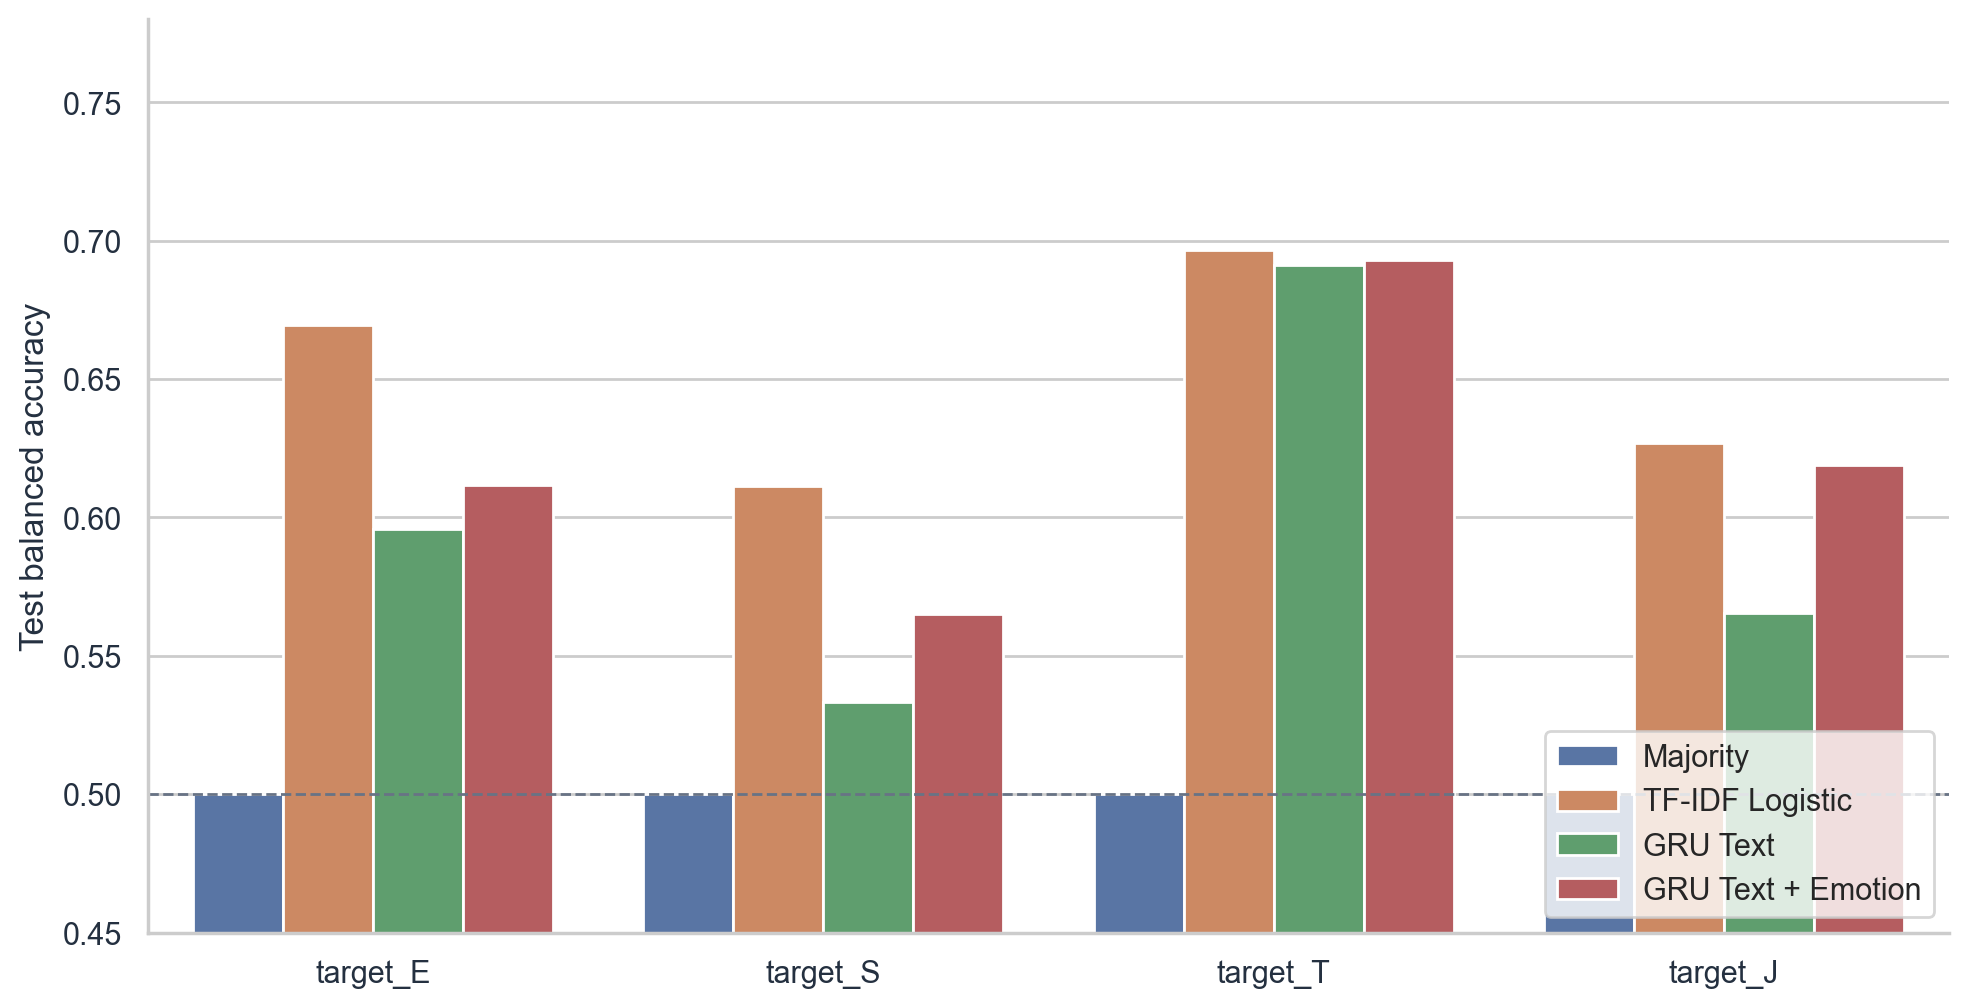
\includegraphics[width=0.85\linewidth]{fig_target_balanced_accuracy.png}
  \caption{Per-dimension test balanced accuracy across baselines. The corrected text-only GRU collapses to majority on $N/S$ and only weakly recovers $E/I$; class-weighted BCE plus author-aggregation pushes TF--IDF and GRU$+$Emotion above $0.5$ on every dimension. Set-attention $P{=}200$ then improves further on every dimension (Appx.~Table~\ref{tab:per-dim}).}
  \label{fig:per-dim}
\end{figure}

\subsection{Does transferred emotion help? A controlled test}\label{sec:emotion}
Three results converge on a cautious answer (Fig.~\ref{fig:emotion-delta}).

\textbf{(i)} \emph{Real emotion vs.\ text}, set-attention $P{=}200$: $\Delta_{\text{real}}{=}{-}0.0069$, $95\%$ CI $[-0.0191, +0.0041]$. The interval covers zero and is slightly negative.

\textbf{(ii)} \emph{Shuffled emotion vs.\ text}: $\Delta_{\text{shuf}}{=}{-}0.0067$, CI $[-0.0200, +0.0052]$. Random author-emotion alignment is statistically indistinguishable from real alignment. This is the negative control: had emotion carried robust author-level signal, $\Delta_{\text{real}}$ would have been clearly above $\Delta_{\text{shuf}}$.

\textbf{(iii)} The \emph{emotion-only} frozen author probe scores $0.565$, above majority ($0.500$) but well below text. Emotion features therefore \emph{do} carry author-level information; they just do not add information that the text encoder has not already captured.

\begin{figure}[t]
  \centering
  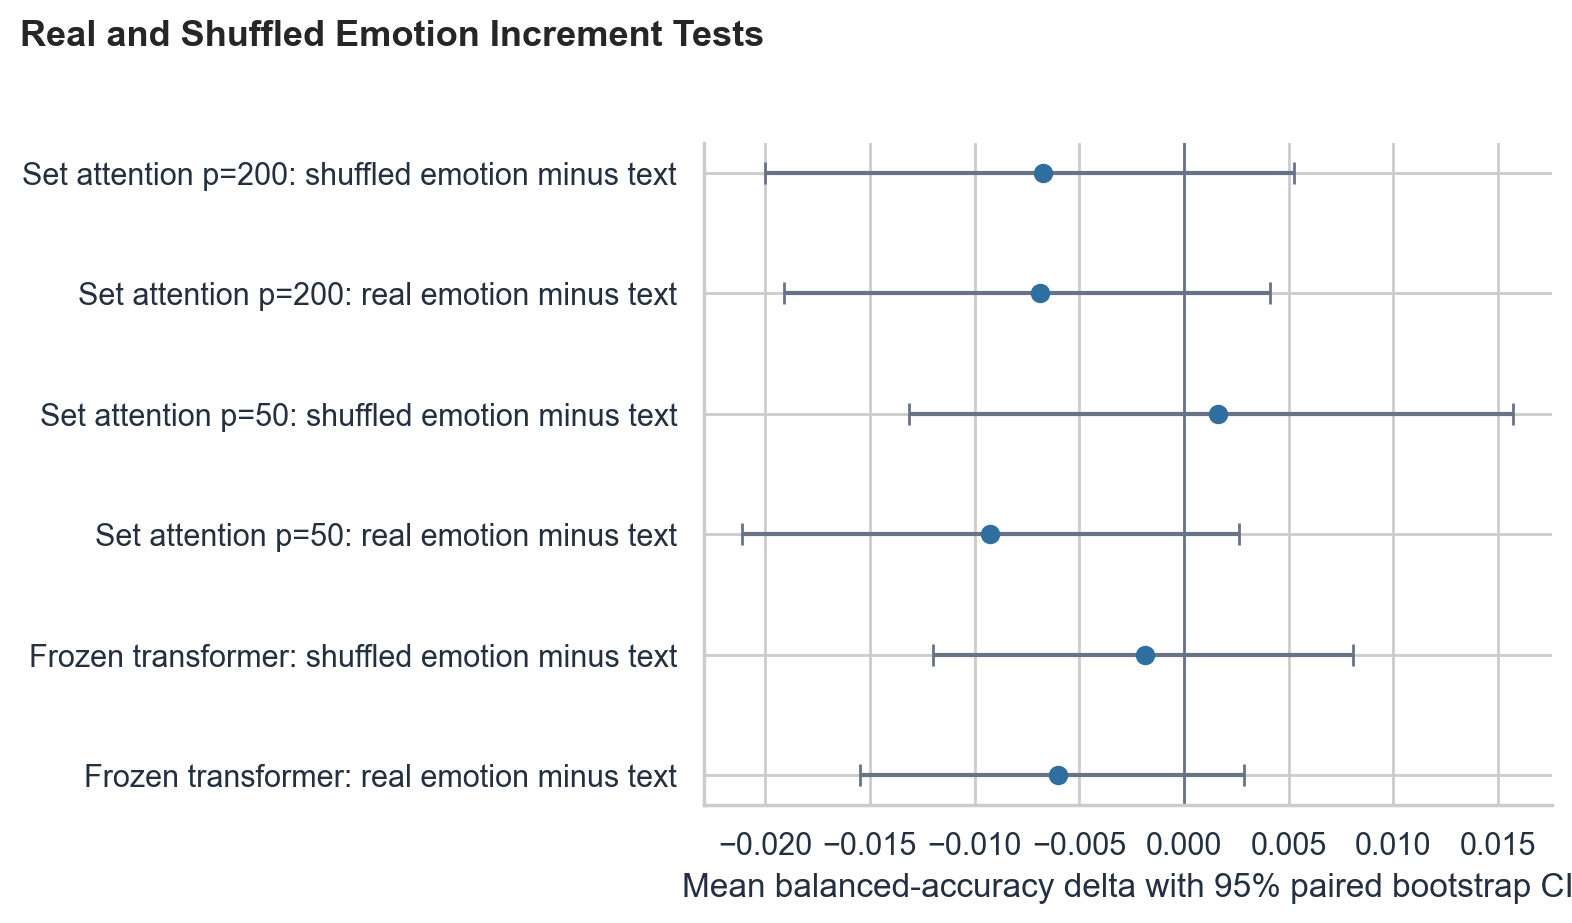
\includegraphics[width=0.78\linewidth]{fig_transformer_emotion_deltas.png}
  \caption{Real-emotion and shuffled-emotion deltas vs.\ text-only, with $95\%$ paired bootstrap CIs over test authors. Across all three families (frozen MiniLM probes, set-attention $P{=}50$, set-attention $P{=}200$), the real-emotion CI overlaps the shuffled-emotion CI and both straddle zero. The negative-control logic implies emotion does \emph{not} add robust incremental signal beyond text.}
  \label{fig:emotion-delta}
\end{figure}

In other words, on this task the marginal information content of $\mathbf{e}_{u,i}$ given $\mathbf{x}_{u,i}$ is near zero. This is consistent with the view that emotion probabilities trained on a small balanced source are largely a low-rank function of the same words MiniLM already encodes.

\subsection{Error structure and stability}
Confusion matrices for set-attention $P{=}200$ (Appx.~Fig.~\ref{fig:cmsa}) show the model still over-predicts the majority class on $S$ (only $74/105$ true $S$ recovered) but recovers $451/621$ true $T$ and $237/334$ true $E$, a qualitatively different error profile from the original GRU baseline (Appx.~Fig.~\ref{fig:cmgru}). Three random seeds give $\mathrm{BA}{=}0.6792\pm 0.0023$ for text-only $P{=}200$ and $0.6732\pm 0.0016$ for the real-emotion variant (Appx.~Fig.~\ref{fig:seed}); $10$- and $20$-epoch caps with early stopping reproduce the same ordering (Appx.~Fig.~\ref{fig:epoch}). Post-budget $P{=}50$ trails $P{=}200$ by $\approx 0.04$ BA, showing that author-level evidence accumulation matters (Appx.~Fig.~\ref{fig:budget}).

\section{Conclusions and discussion}

\textbf{What we claim.} (1) Predicting MBTI from Reddit writing should be done at the author level; post-level random splits and post-level metrics inflate results. (2) A single block of multi-head self-attention over the unordered set of an author's masked post embeddings is, on this corpus, a stronger model than TF--IDF logistic regression and substantially stronger than corrected GRU baselines. (3) Transferred emotion probabilities are informative on their own but \emph{do not} robustly add to text representations, as evidenced by overlapping real-vs-shuffled emotion deltas.

\textbf{What we do not claim.} We do not claim emotion features are useless in general. Only conditional on a sufficiently expressive frozen text encoder and author-level aggregation, the emotion-specific increment is within seed/control noise on this Reddit corpus. We make no causal claim about a user's mood; $\mathbf{e}_{u,i}$ is a transferred text-derived representation.

\textbf{Limitations.} (a) MBTI labels are self-reported in a known online community and may correlate with stylistic markers irrelevant to personality. (b) The post-budget hash is a stable but non-temporal sampler; truly chronological models could recover longitudinal effects. (c) Our frozen encoder is MiniLM; supervised post-level transformer fine-tuning could change the picture but reintroduces post-label noise and was intentionally excluded. (d) The emotion-balanced source is small and English-only.

\textbf{Future work.} A natural next step is to replace the per-post emotion classifier with a low-rank residual on top of MiniLM, which would test whether emotion adds anything specifically orthogonal to text. A second direction is to expand the set-attention block into a Set Transformer with inducing points~\citep{lee2019settransformer} to scale beyond $P{=}200$.

\section{Broader impact}

Personality inference from public writing is dual-use. Beneficial applications include support-line triage and pedagogically adaptive systems. Concrete harms include profiling without consent, targeted manipulation in advertising, and use in hiring or housing decisions where MBTI lacks predictive validity~\citep{pittenger1993utility}. Our author-level frame and controlled emotion test are intended to make the gap between ``learnable'' and ``meaningful'' more visible: even our best model has mean balanced accuracy below $0.7$ and recovers only $\approx 70\%$ of minority $S$/$E$ labels, which we would consider far too noisy for any consequential decision about an individual.

{\small
\bibliographystyle{plainnat}
\begin{thebibliography}{99}

\bibitem[Devlin et~al.(2019)]{devlin2019bert}
J.~Devlin, M.-W.~Chang, K.~Lee, and K.~Toutanova.
\newblock BERT: Pre-training of Deep Bidirectional Transformers for Language Understanding.
\newblock In \emph{NAACL}, 2019.

\bibitem[Gjurkovi\'c and \v{S}najder(2018)]{gjurkovic2018reddit}
M.~Gjurkovi\'c and J.~\v{S}najder.
\newblock Reddit: A Gold Mine for Personality Prediction.
\newblock In \emph{Proceedings of the Second Workshop on Computational Modeling of People's Opinions, Personality, and Emotions in Social Media}, 2018.

\bibitem[Hugging Face emotion-balanced(2023)]{hf_emotion_balanced}
AdamCodd.
\newblock \texttt{AdamCodd/emotion-balanced} Hugging Face dataset.
\newblock \url{https://huggingface.co/datasets/AdamCodd/emotion-balanced}.

\bibitem[Kaggle Reddit MBTI(2024)]{kaggle_reddit_mbti}
M.~Zhang.
\newblock \texttt{minhaozhang1/reddit-mbti-dataset} on Kaggle.
\newblock \url{https://www.kaggle.com/datasets/minhaozhang1/reddit-mbti-dataset}, 2024.

\bibitem[Lee et~al.(2019)]{lee2019settransformer}
J.~Lee, Y.~Lee, J.~Kim, A.~Kosiorek, S.~Choi, and Y.~W. Teh.
\newblock Set Transformer: A Framework for Attention-Based Permutation-Invariant Neural Networks.
\newblock In \emph{ICML}, 2019.

\bibitem[Mairesse et~al.(2007)]{mairesse2007using}
F.~Mairesse, M.~Walker, M.~Mehl, and R.~Moore.
\newblock Using Linguistic Cues for the Automatic Recognition of Personality in Conversation and Text.
\newblock \emph{JAIR}, 30:457--500, 2007.

\bibitem[Park et~al.(2015)]{park2015automatic}
G.~Park, H.~A.~Schwartz, J.~C.~Eichstaedt, M.~L.~Kern, M.~Kosinski, D.~J.~Stillwell, L.~H.~Ungar, and M.~E.~P.~Seligman.
\newblock Automatic Personality Assessment Through Social Media Language.
\newblock \emph{J.\ Personality and Social Psychology}, 108(6):934--952, 2015.

\bibitem[Pennebaker and King(1999)]{pennebaker1999linguistic}
J.~W. Pennebaker and L.~A. King.
\newblock Linguistic Styles: Language Use as an Individual Difference.
\newblock \emph{J.\ Personality and Social Psychology}, 77(6):1296--1312, 1999.

\bibitem[Pittenger(1993)]{pittenger1993utility}
D.~J. Pittenger.
\newblock The Utility of the Myers--Briggs Type Indicator.
\newblock \emph{Review of Educational Research}, 63(4):467--488, 1993.

\bibitem[Plank and Hovy(2015)]{plank2015personality}
B.~Plank and D.~Hovy.
\newblock Personality Traits on Twitter---or---How to Get 1,500 Personality Tests in a Week.
\newblock In \emph{WASSA}, 2015.

\bibitem[Reimers and Gurevych(2019)]{reimers2019sentencebert}
N.~Reimers and I.~Gurevych.
\newblock Sentence-BERT: Sentence Embeddings using Siamese BERT-Networks.
\newblock In \emph{EMNLP}, 2019.

\bibitem[Vaswani et~al.(2017)]{vaswani2017attention}
A.~Vaswani et~al.
\newblock Attention Is All You Need.
\newblock In \emph{NeurIPS}, 2017.

\bibitem[Wang et~al.(2020)]{wang2020minilm}
W.~Wang, F.~Wei, L.~Dong, H.~Bao, N.~Yang, and M.~Zhou.
\newblock MiniLM: Deep Self-Attention Distillation for Task-Agnostic Compression of Pre-Trained Transformers.
\newblock In \emph{NeurIPS}, 2020.

\bibitem[Zaheer et~al.(2017)]{zaheer2017deepsets}
M.~Zaheer, S.~Kottur, S.~Ravanbakhsh, B.~P\'oczos, R.~Salakhutdinov, and A.~Smola.
\newblock Deep Sets.
\newblock In \emph{NeurIPS}, 2017.

\bibitem[Cursor / Anthropic(2026)]{cursor_ai}
Cursor IDE with Anthropic Claude.
\newblock Used for code completion, refactoring suggestions, and report copy-editing. All numerical results were verified against tracked CSV artifacts in the project's \texttt{report/results/} directory.

\end{thebibliography}
}

\newpage
\appendix

\section{Appendix: supplementary figures and tables}

This appendix collects supporting EDA visuals, sensitivity studies, and per-dimension breakdowns that support but are not required for the main argument.

\subsection{Token length and emotion-transfer EDA}

\begin{figure}[H]
  \centering
  \begin{subfigure}[t]{0.48\linewidth}
    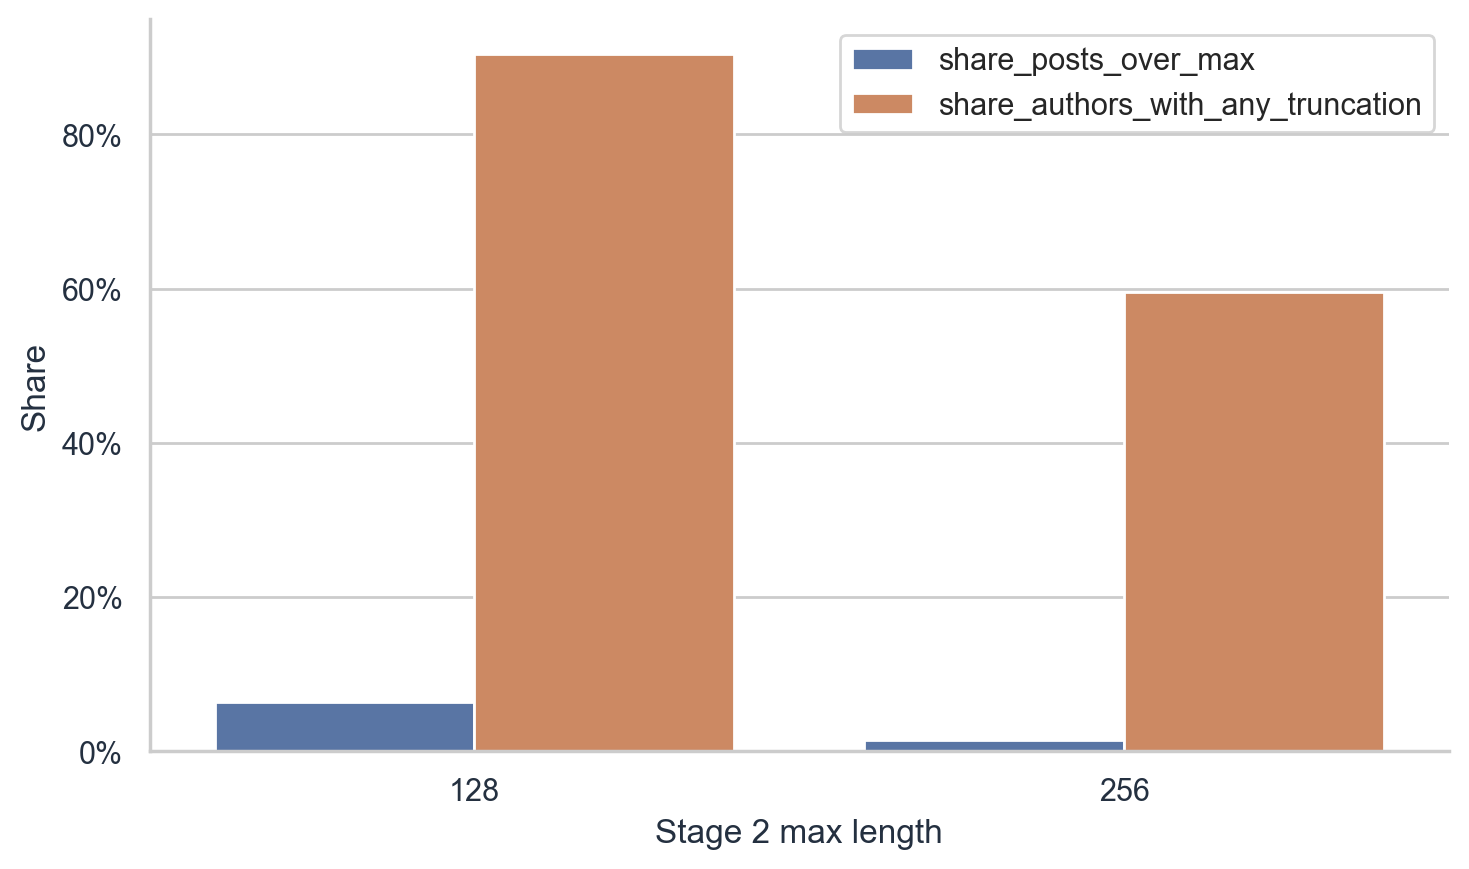
\includegraphics[width=\linewidth]{fig_token_length_sensitivity.png}
    \caption{Token-length sensitivity for 128- vs.\ 256-token caps. The 256 cap truncates only $1.5\%$ of posts (vs.\ $6.4\%$ at 128), motivating its use for MiniLM.}
    \label{fig:tokenlen}
  \end{subfigure}
  \hfill
  \begin{subfigure}[t]{0.48\linewidth}
    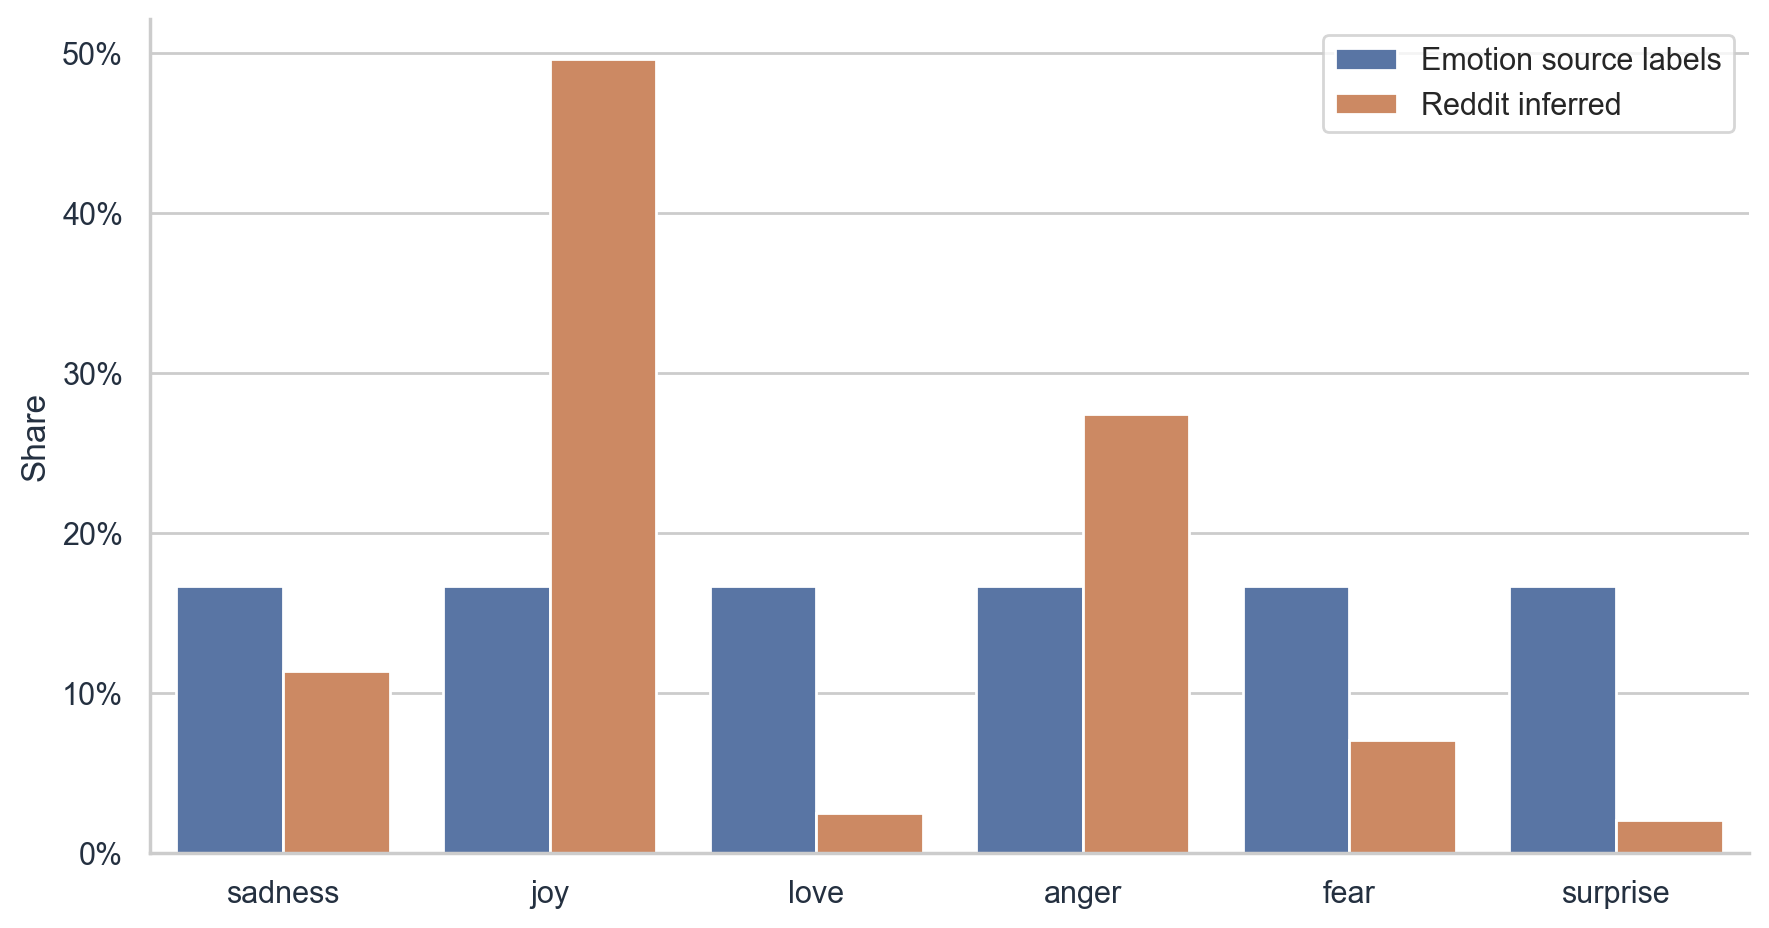
\includegraphics[width=\linewidth]{fig_source_vs_reddit_emotion_distribution.png}
    \caption{Source emotion-balanced labels vs.\ Reddit-inferred posterior shares. Reddit posts skew toward joy and anger; this is why we treat emotion as a transferred representation rather than a calibrated mood measurement.}
    \label{fig:emotiondist}
  \end{subfigure}
  \caption{Token-length and emotion-distribution EDA used to motivate modelling choices.}
\end{figure}

\begin{figure}[H]
  \centering
  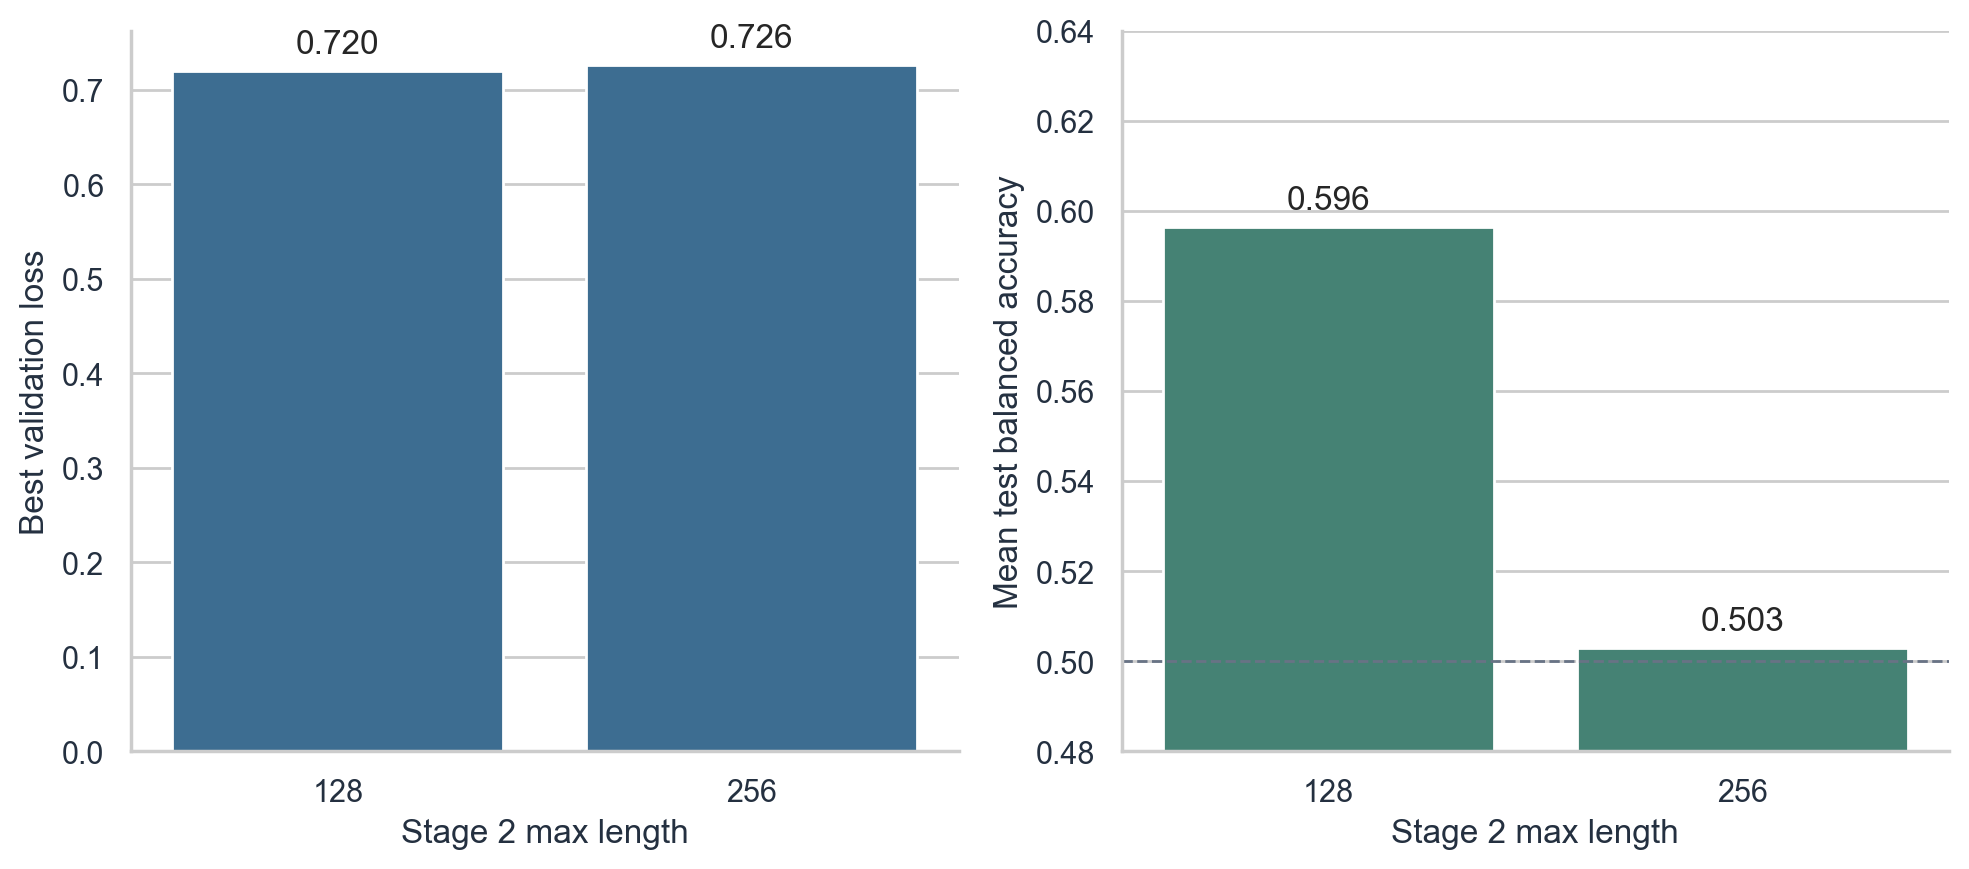
\includegraphics[width=0.7\linewidth]{fig_max_length_training_sensitivity.png}
  \caption{Stage~2 GRU training sensitivity to maximum sequence length. The 128-token GRU is what we report as the baseline; the 256-token GRU collapsed during full training, suggesting that the GRU+embedding combination does not benefit from longer truncation without further regularisation.}
  \label{fig:maxlen}
\end{figure}

\subsection{Baseline and GRU diagnostics}

\begin{figure}[H]
  \centering
  \begin{subfigure}[t]{0.48\linewidth}
    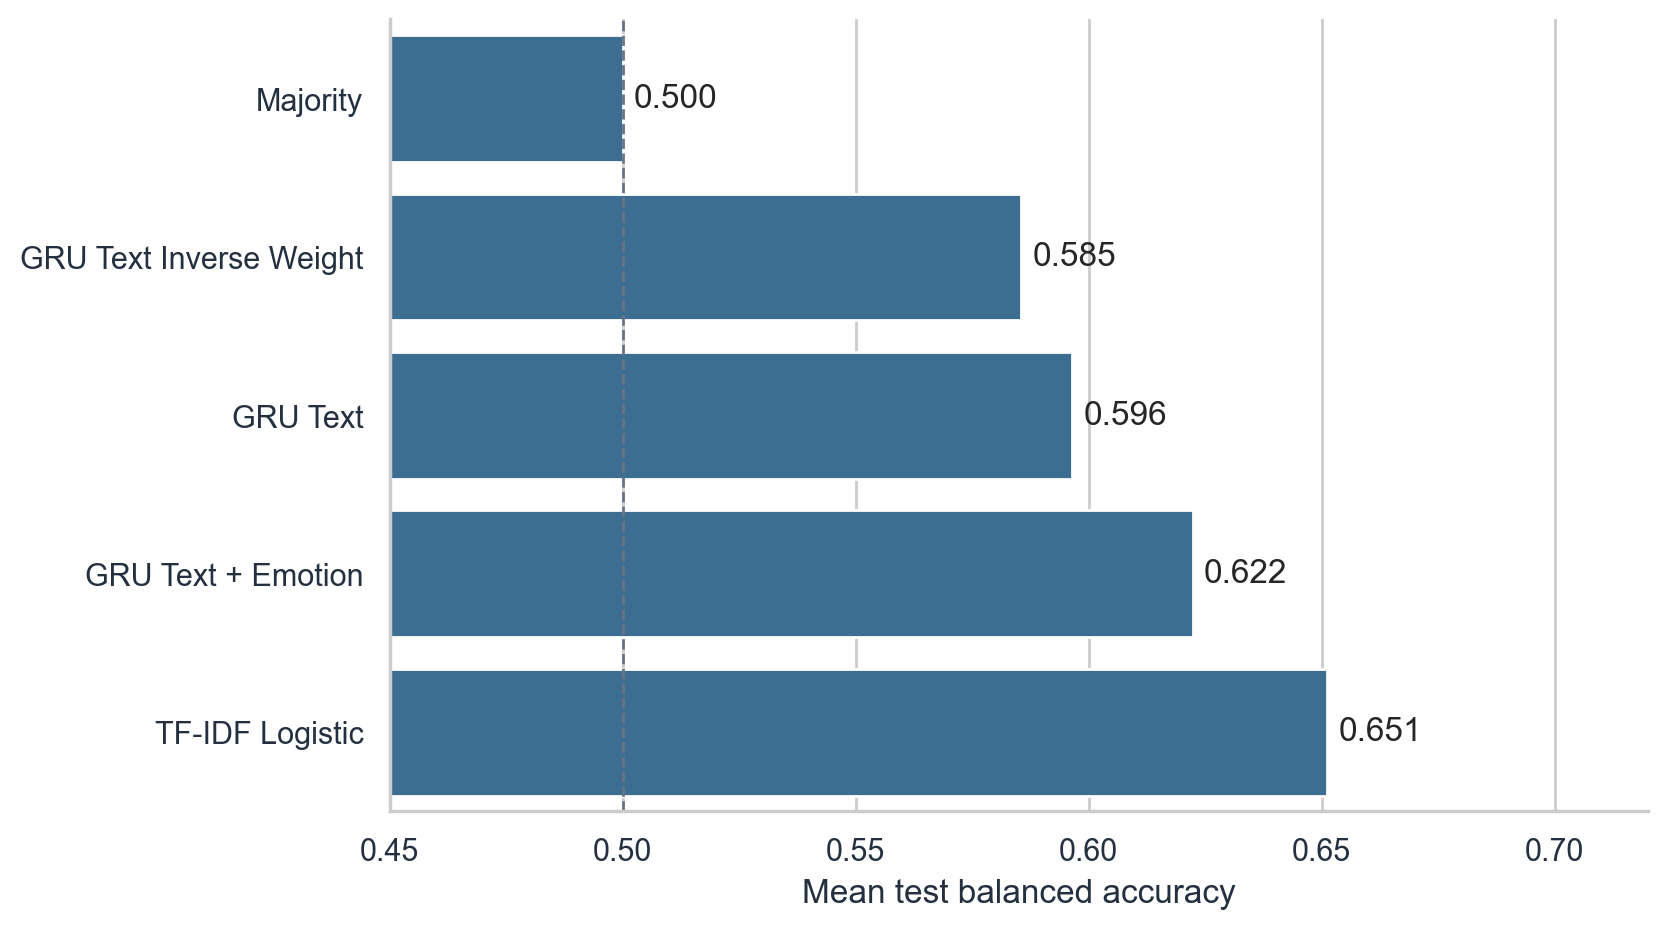
\includegraphics[width=\linewidth]{fig_model_summary_balanced_accuracy.png}
    \caption{Baseline mean test balanced accuracy across the five non-transformer models.}
  \end{subfigure}
  \hfill
  \begin{subfigure}[t]{0.48\linewidth}
    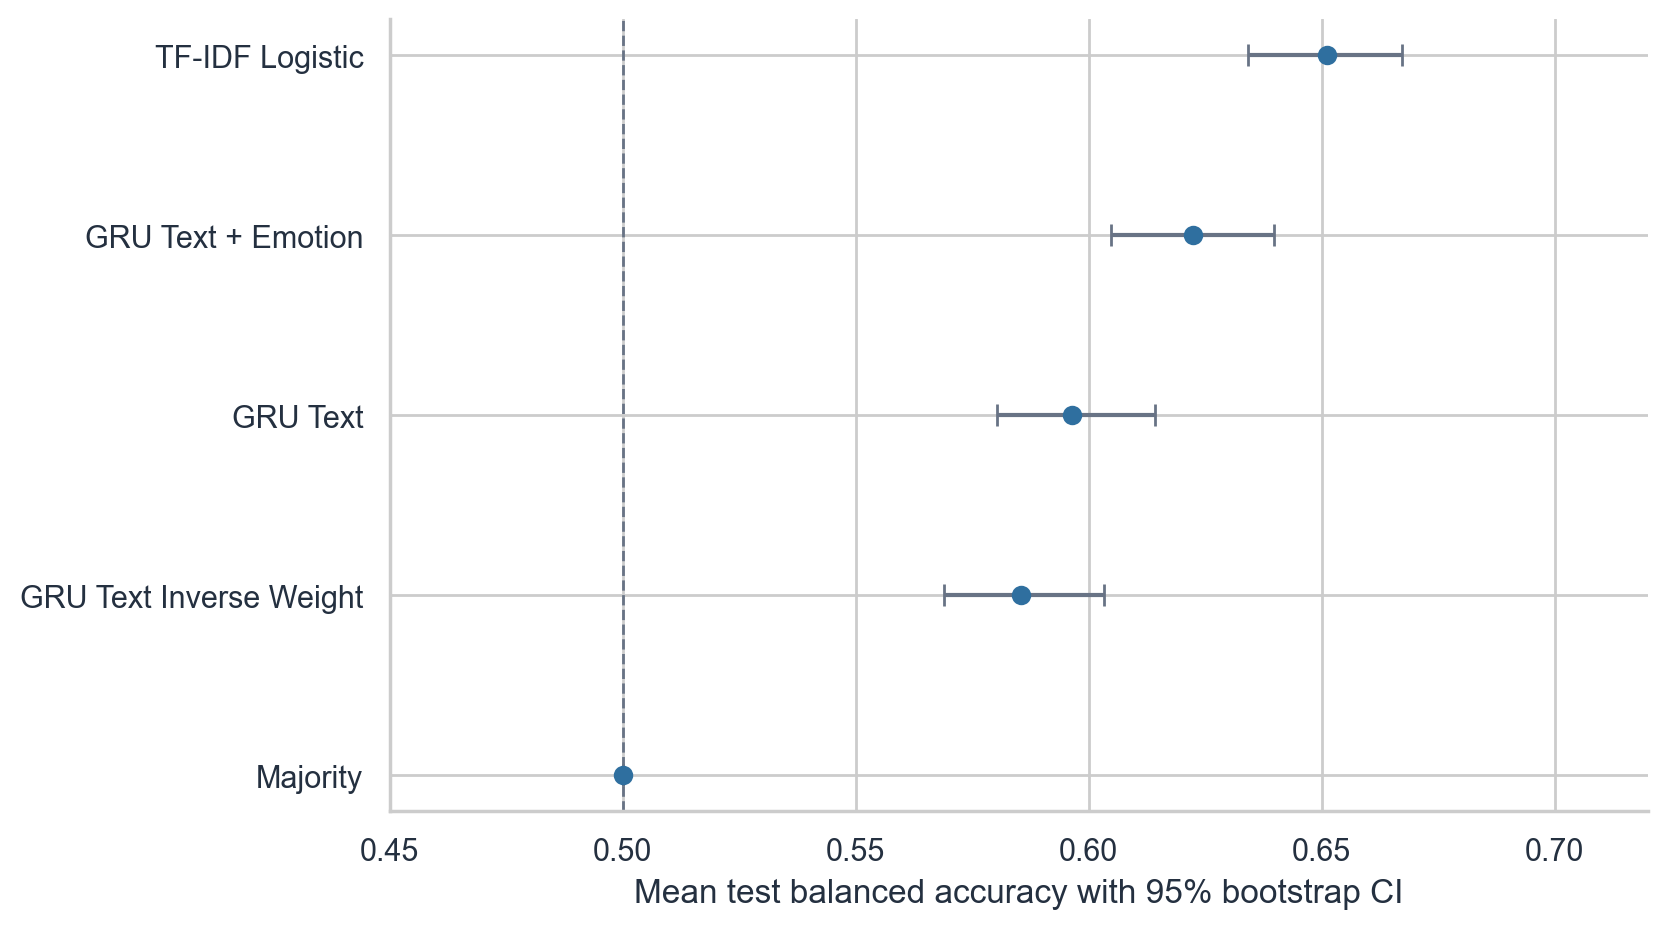
\includegraphics[width=\linewidth]{fig_bootstrap_balanced_accuracy_ci.png}
    \caption{$95\%$ bootstrap CIs ($B{=}2000$, test authors) for the five baselines.}
  \end{subfigure}
  \caption{Baseline mean test balanced accuracy and bootstrap CIs. Set-attention models are excluded here; see Fig.~\ref{fig:summary} for them.}
\end{figure}

\begin{figure}[H]
  \centering
  \begin{subfigure}[t]{0.48\linewidth}
    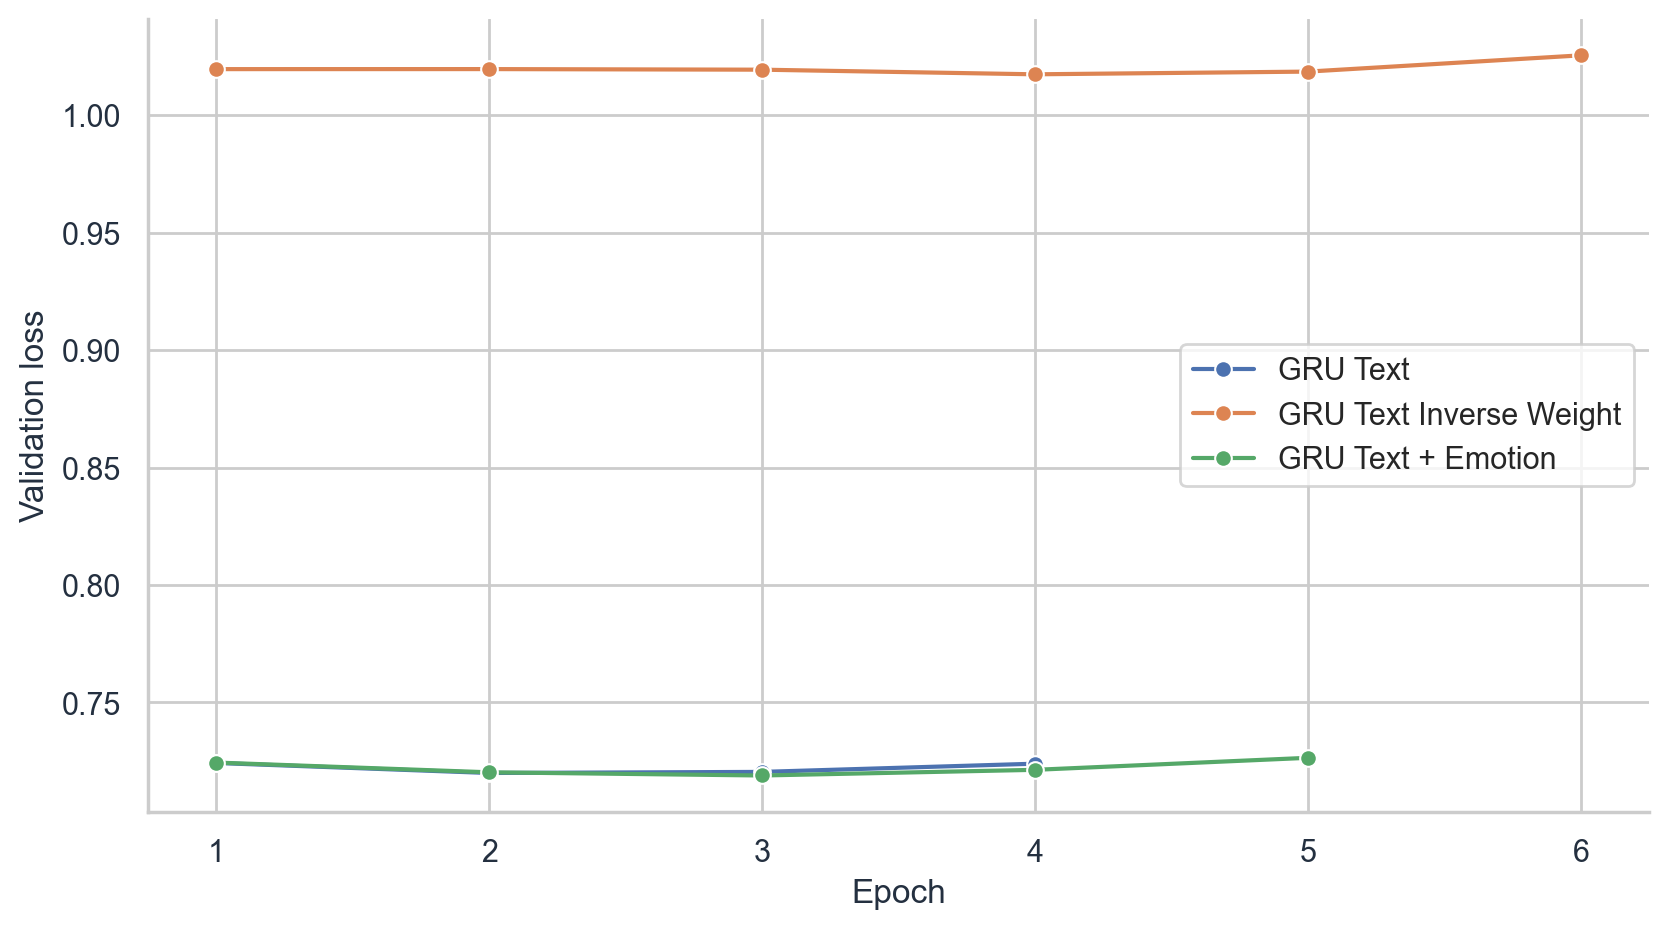
\includegraphics[width=\linewidth]{fig_gru_validation_loss.png}
    \caption{Stage~2 GRU validation BCE over epochs. The text$+$emotion variant tracks text-only closely.}
  \end{subfigure}
  \hfill
  \begin{subfigure}[t]{0.48\linewidth}
    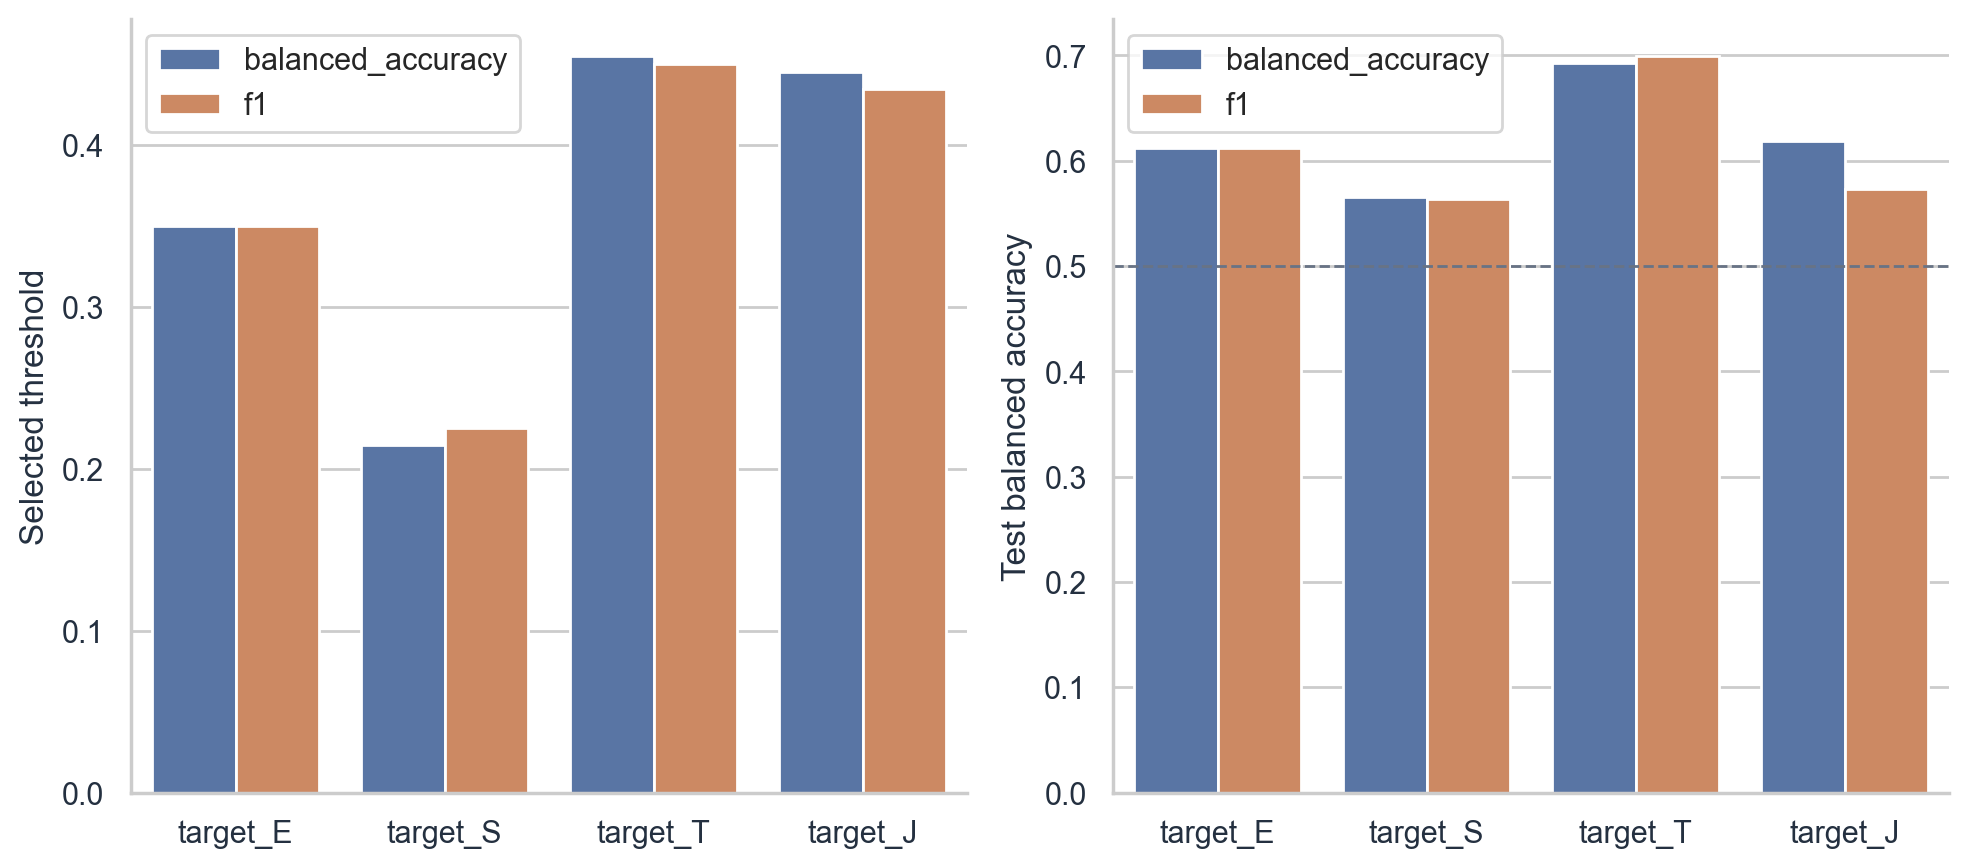
\includegraphics[width=\linewidth]{fig_threshold_objective_sensitivity.png}
    \caption{Threshold objective sensitivity: tuning for balanced accuracy vs.\ F1 yields very similar test BA but different F1.}
  \end{subfigure}
  \caption{Corrected GRU diagnostics underlying the baseline rows of Table~\ref{tab:main}.}
\end{figure}

\begin{figure}[H]
  \centering
  \begin{subfigure}[t]{0.55\linewidth}
    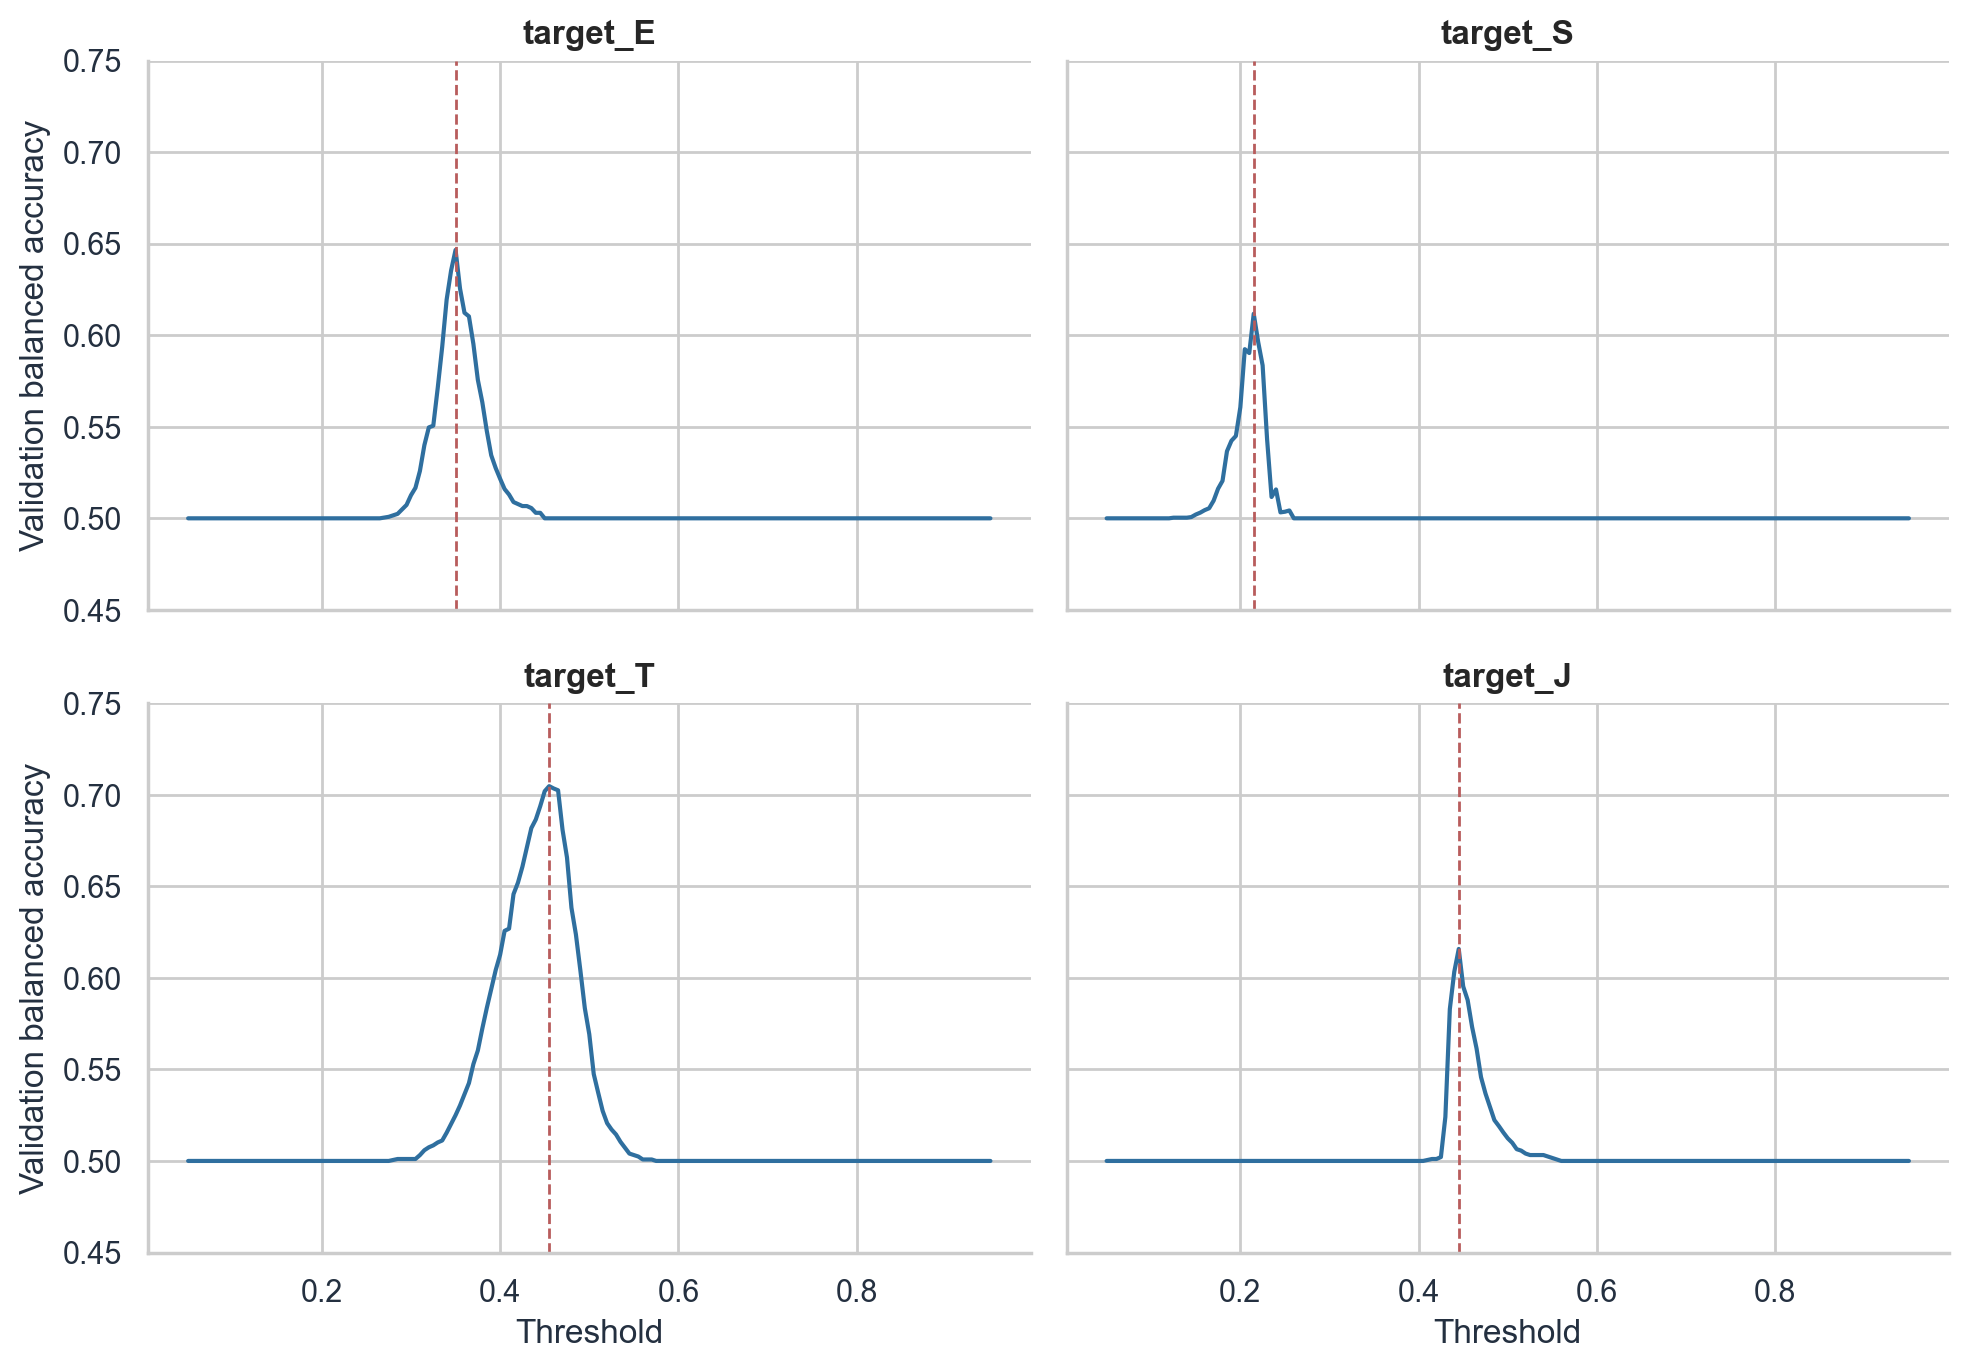
\includegraphics[width=\linewidth]{fig_final_threshold_tuning_curves.png}
    \caption{Validation balanced-accuracy curves over the threshold grid for the corrected text$+$emotion GRU. Tuned thresholds are far from $0.5$ for the imbalanced $S$ and $E$ dimensions.}
  \end{subfigure}
  \hfill
  \begin{subfigure}[t]{0.42\linewidth}
    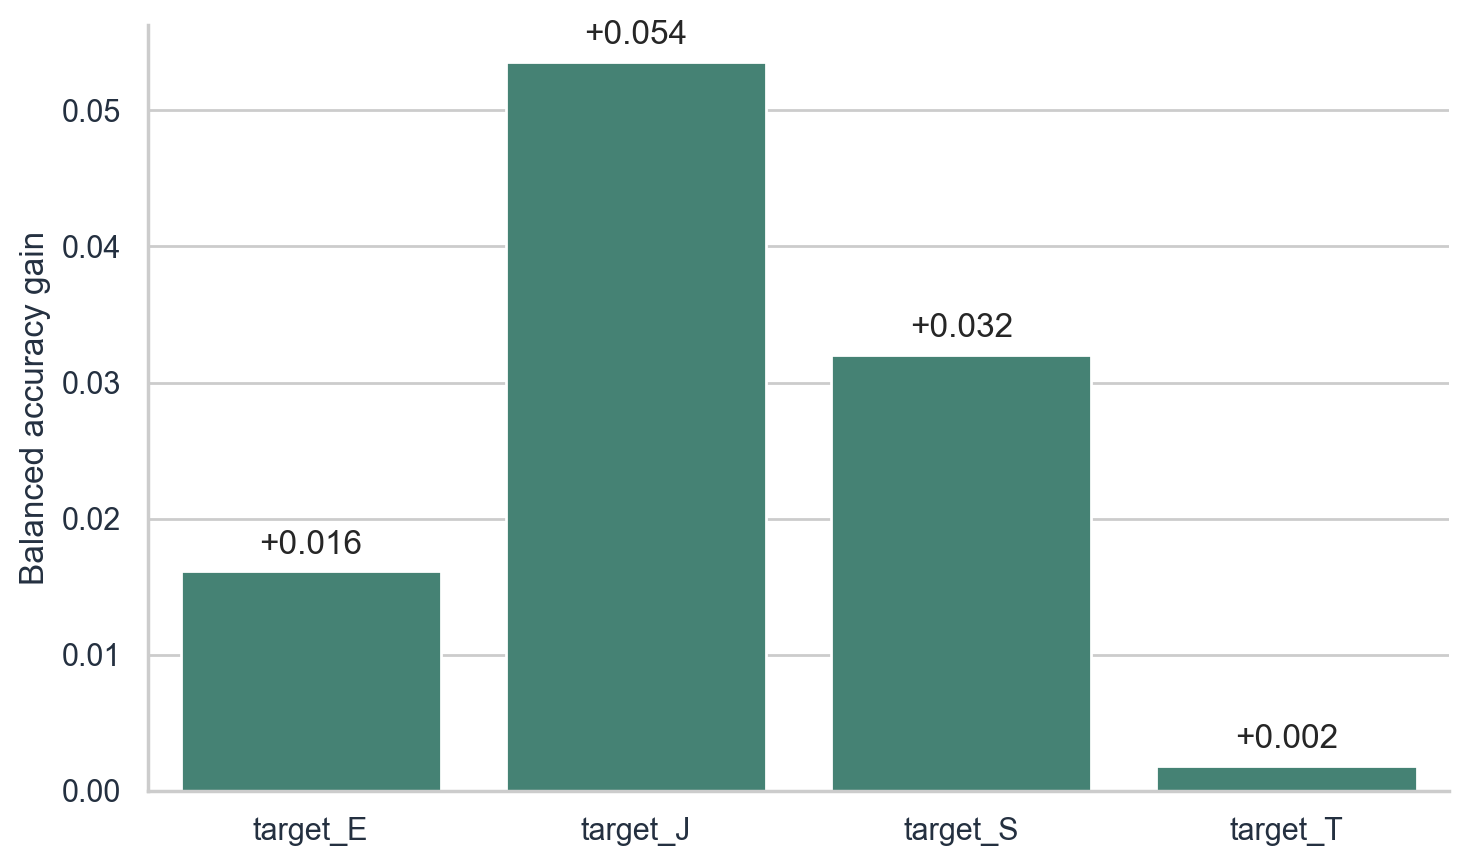
\includegraphics[width=\linewidth]{fig_emotion_gain_by_target.png}
    \caption{Per-dimension GRU emotion gain (text$+$emotion minus text-only); the transformer control test in Fig.~\ref{fig:emotion-delta} retracts these gains once a stronger text encoder is used.}
  \end{subfigure}
  \caption{Threshold tuning and per-dimension GRU emotion gain diagnostics.}
\end{figure}

\subsection{Per-dimension headline metrics}

\begin{table}[H]
\small
\centering
\caption{Per-dimension test balanced accuracy for selected models. Set-attention $P{=}200$ improves every dimension over the corrected GRU and improves $E$, $S$, and $T$ over TF--IDF.}
\label{tab:per-dim}
\begin{tabular}{lrrrr}
\toprule
Model & $E/I$ & $N/S$ & $F/T$ & $J/P$ \\
\midrule
GRU Text                              & 0.596 & 0.533 & 0.691 & 0.566 \\
GRU Text $+$ Emotion                  & 0.612 & 0.565 & 0.693 & 0.619 \\
TF--IDF Logistic                      & 0.669 & 0.611 & 0.697 & 0.627 \\
Set Attention Text $P{=}200$          & 0.691 & 0.672 & 0.732 & 0.640 \\
Set Attention Text $+$ Real Emo. $P{=}200$ & 0.676 & 0.666 & 0.723 & 0.642 \\
Set Attention Text $+$ Controls $P{=}200$ & 0.691 & 0.672 & 0.731 & 0.657 \\
\bottomrule
\end{tabular}
\end{table}

\subsection{Set-attention error structure and stability}

\begin{figure}[H]
  \centering
  \begin{subfigure}[t]{0.48\linewidth}
    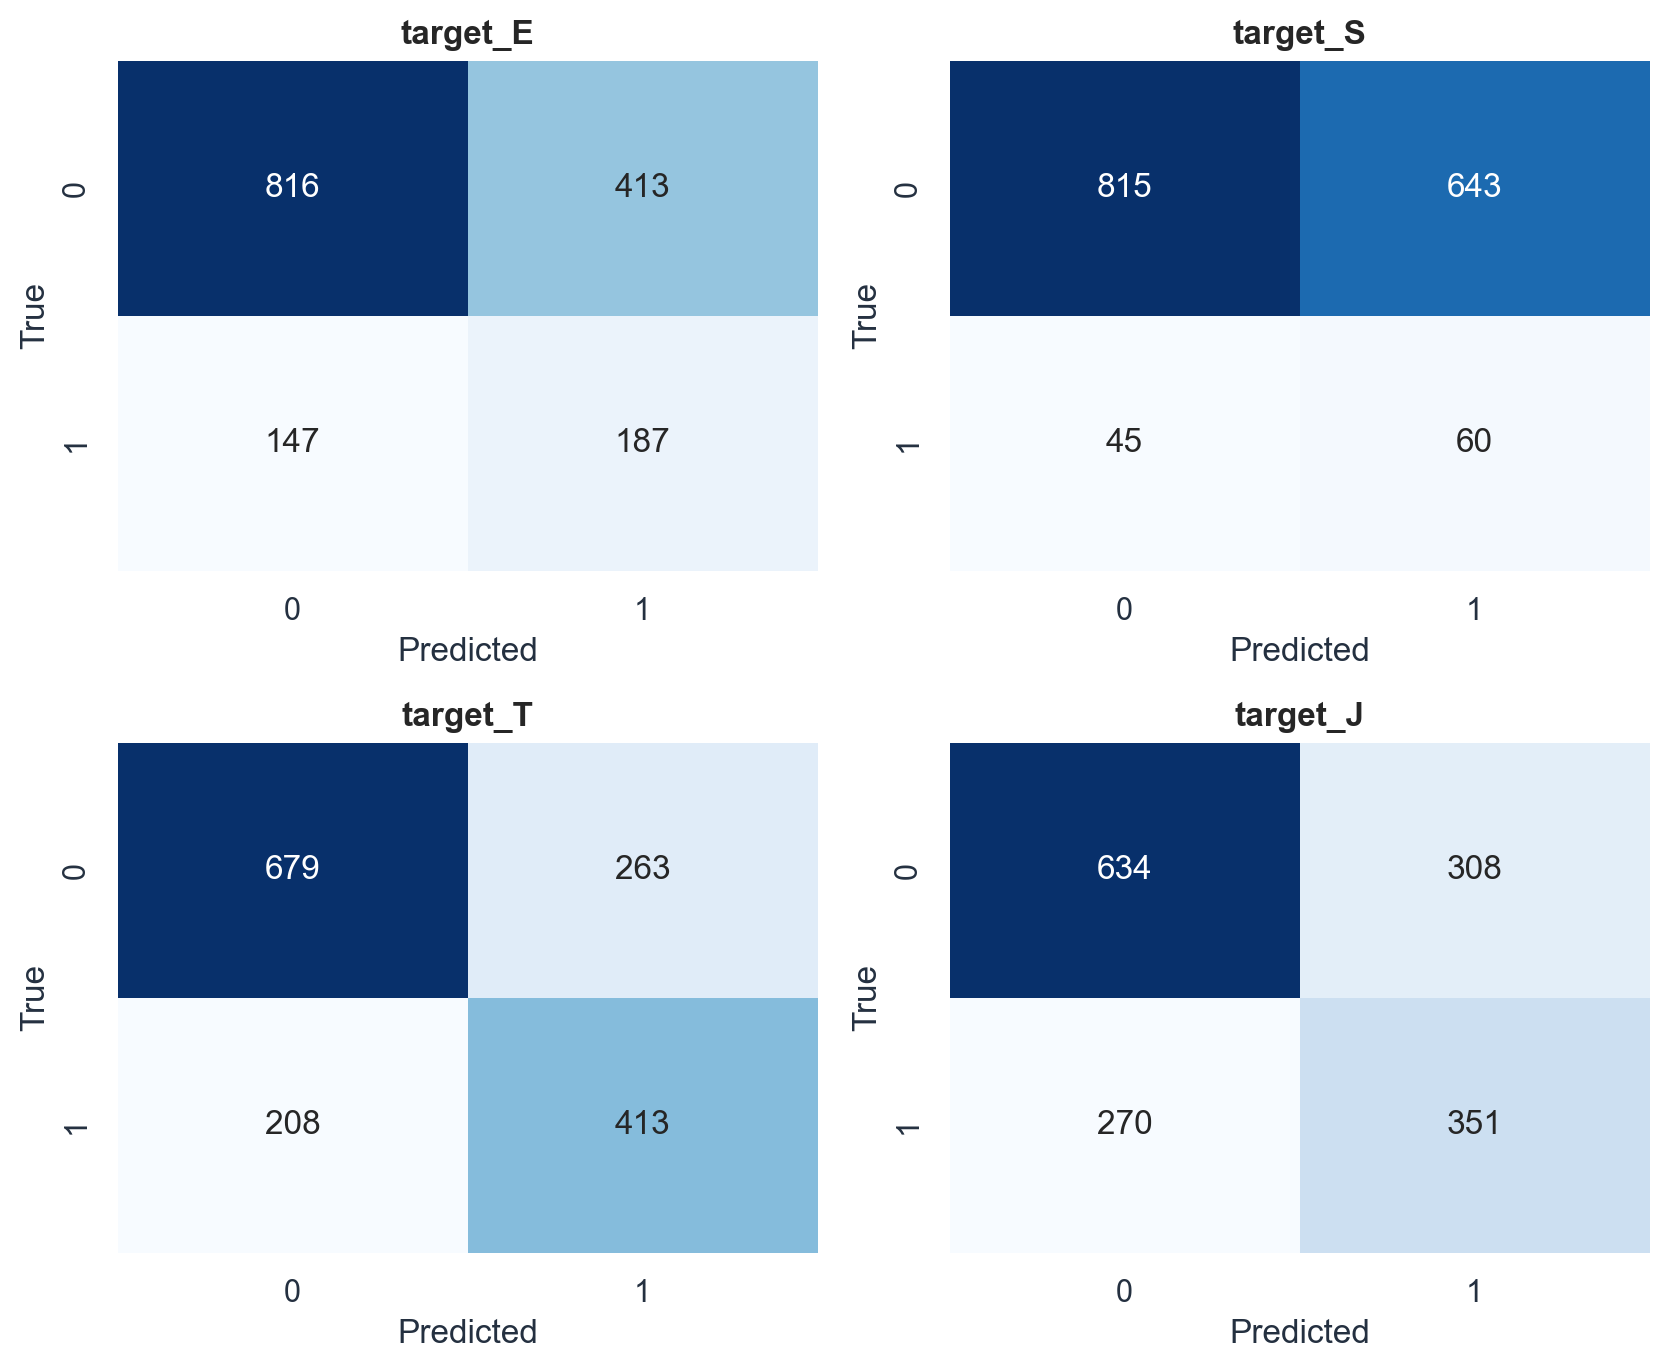
\includegraphics[width=\linewidth]{fig_gru_baseline_confusion_matrices.png}
    \caption{Corrected GRU text$+$emotion confusion matrices.}
    \label{fig:cmgru}
  \end{subfigure}
  \hfill
  \begin{subfigure}[t]{0.48\linewidth}
    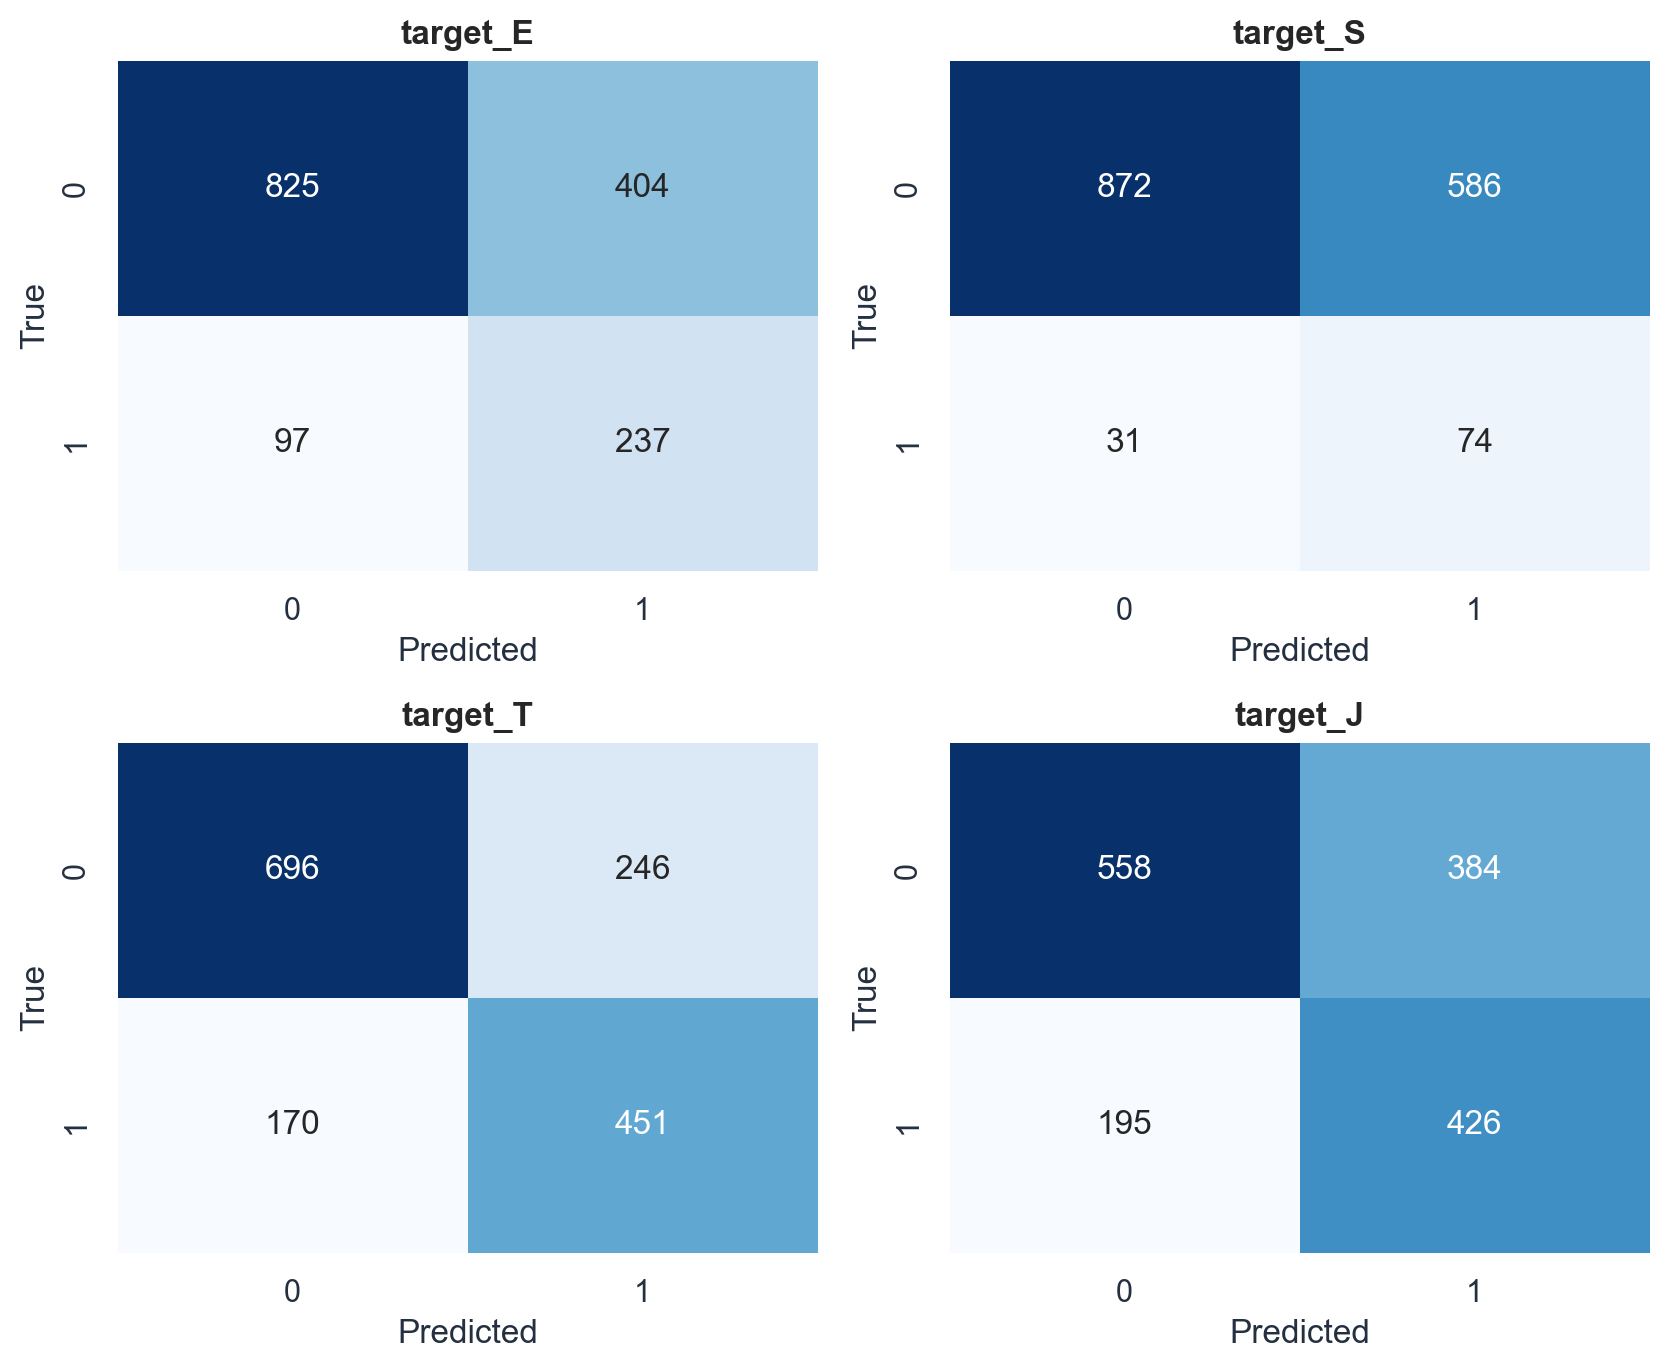
\includegraphics[width=\linewidth]{fig_set_attention_p200_confusion_matrices.png}
    \caption{Set-attention text $P{=}200$ confusion matrices.}
    \label{fig:cmsa}
  \end{subfigure}
  \caption{Per-dimension confusion structure. Set-attention recovers minority $S$, $E$ at a much higher rate than the GRU.}
\end{figure}

\begin{figure}[H]
  \centering
  \begin{subfigure}[t]{0.31\linewidth}
    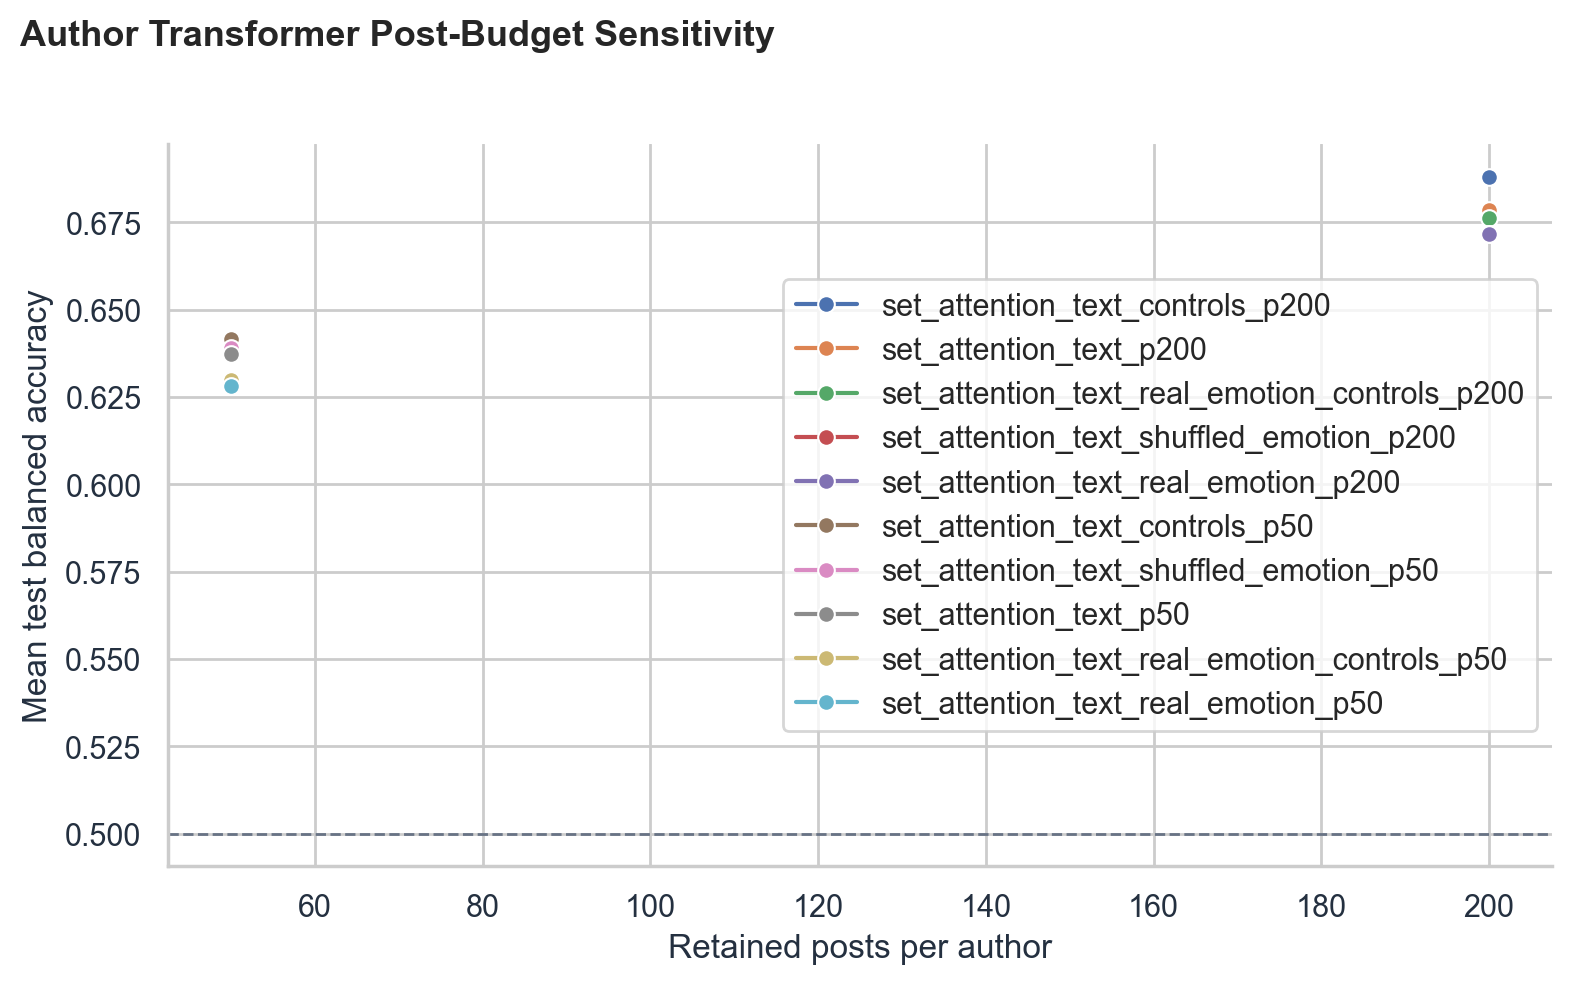
\includegraphics[width=\linewidth]{fig_set_attention_post_budget.png}
    \caption{Post-budget sensitivity ($P{=}50$ vs.\ $P{=}200$).}
    \label{fig:budget}
  \end{subfigure}
  \hfill
  \begin{subfigure}[t]{0.31\linewidth}
    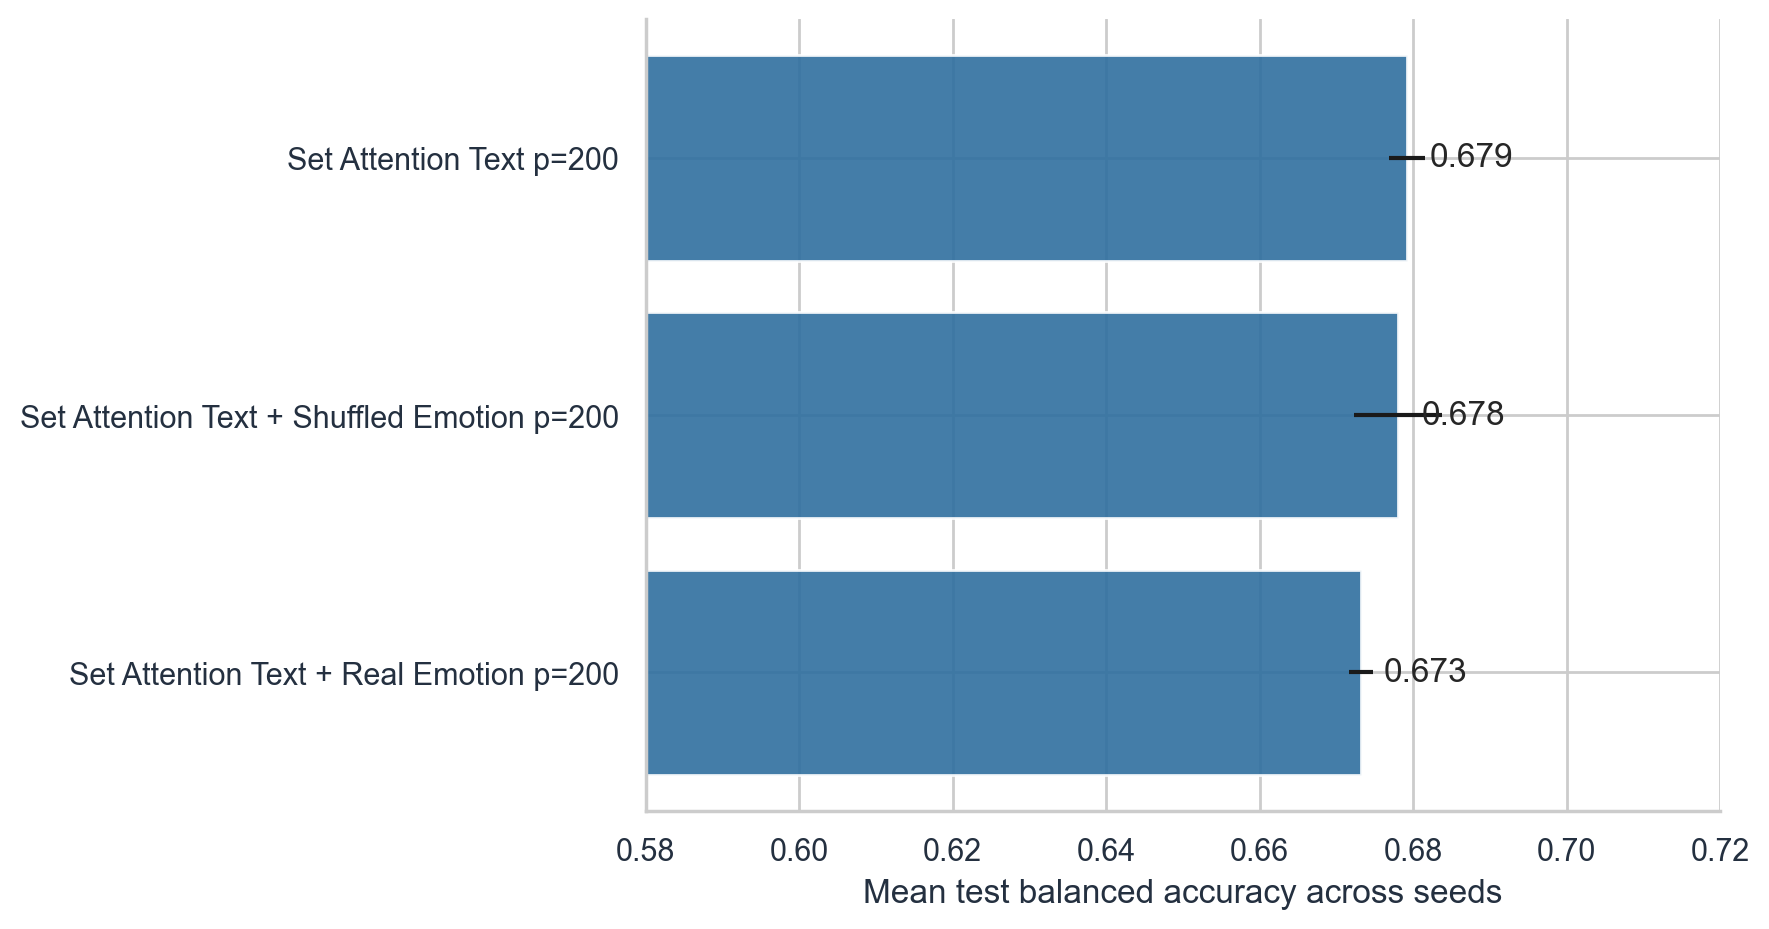
\includegraphics[width=\linewidth]{fig_set_attention_seed_stability.png}
    \caption{Seed stability across three random seeds.}
    \label{fig:seed}
  \end{subfigure}
  \hfill
  \begin{subfigure}[t]{0.31\linewidth}
    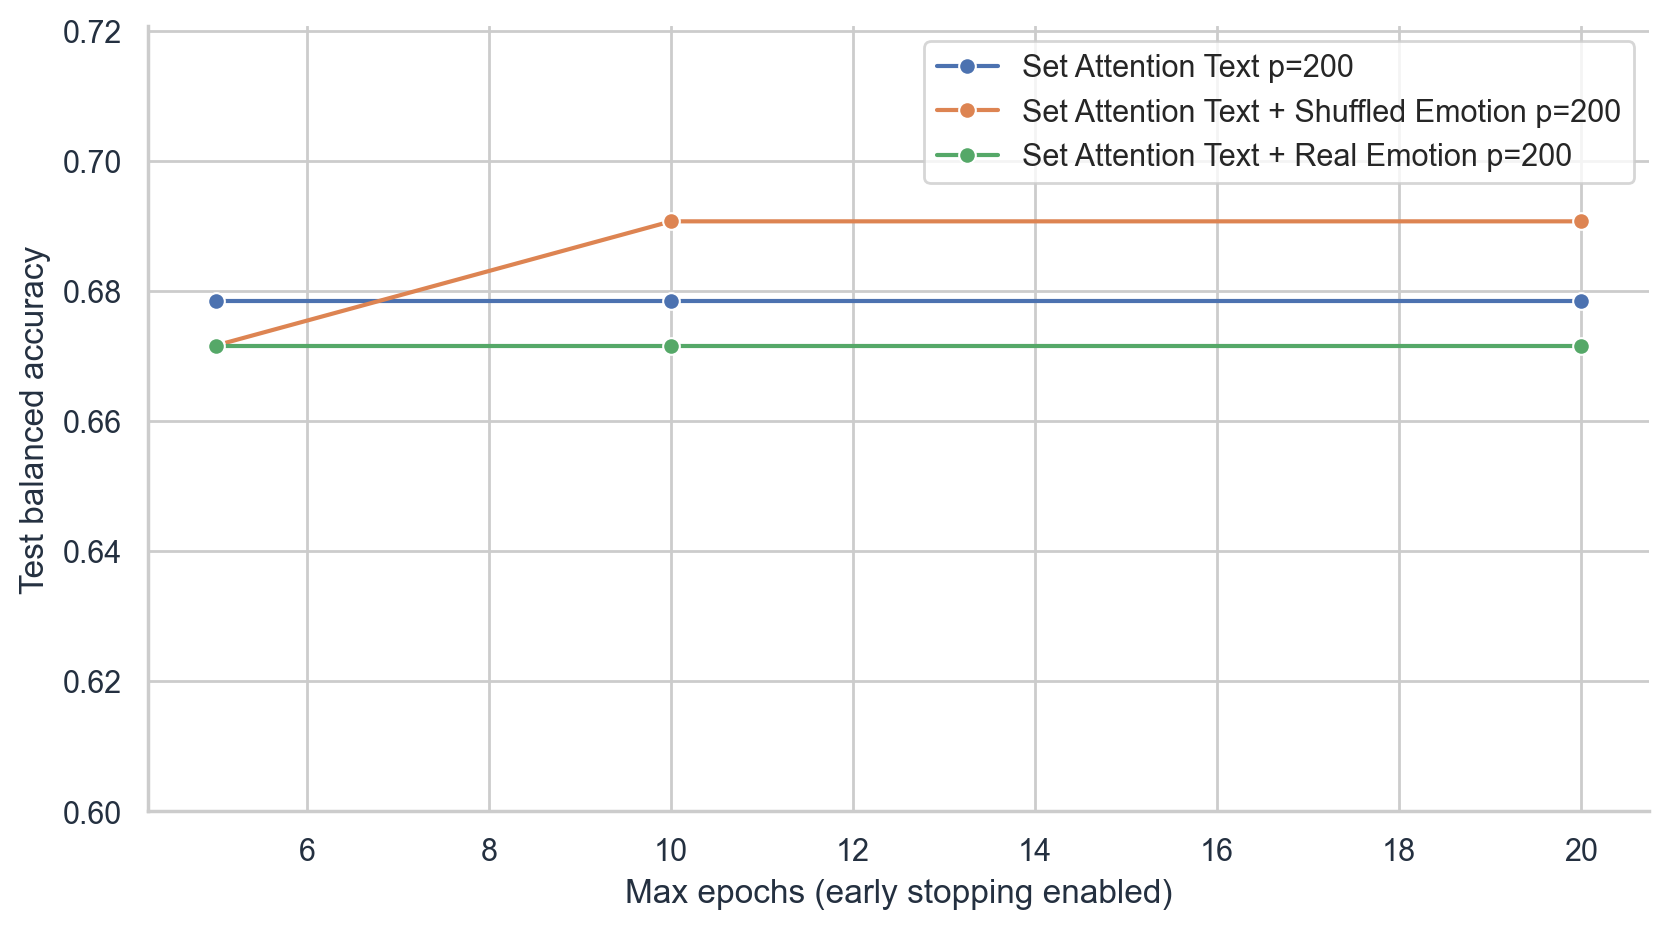
\includegraphics[width=\linewidth]{fig_set_attention_epoch_sensitivity.png}
    \caption{Epoch-cap sensitivity ($5$/$10$/$20$ epochs, early stopping enabled).}
    \label{fig:epoch}
  \end{subfigure}
  \caption{Set-attention $P{=}200$ stability checks. The author-level direction is stable across post budget, seed, and epoch cap.}
\end{figure}

\begin{figure}[H]
  \centering
  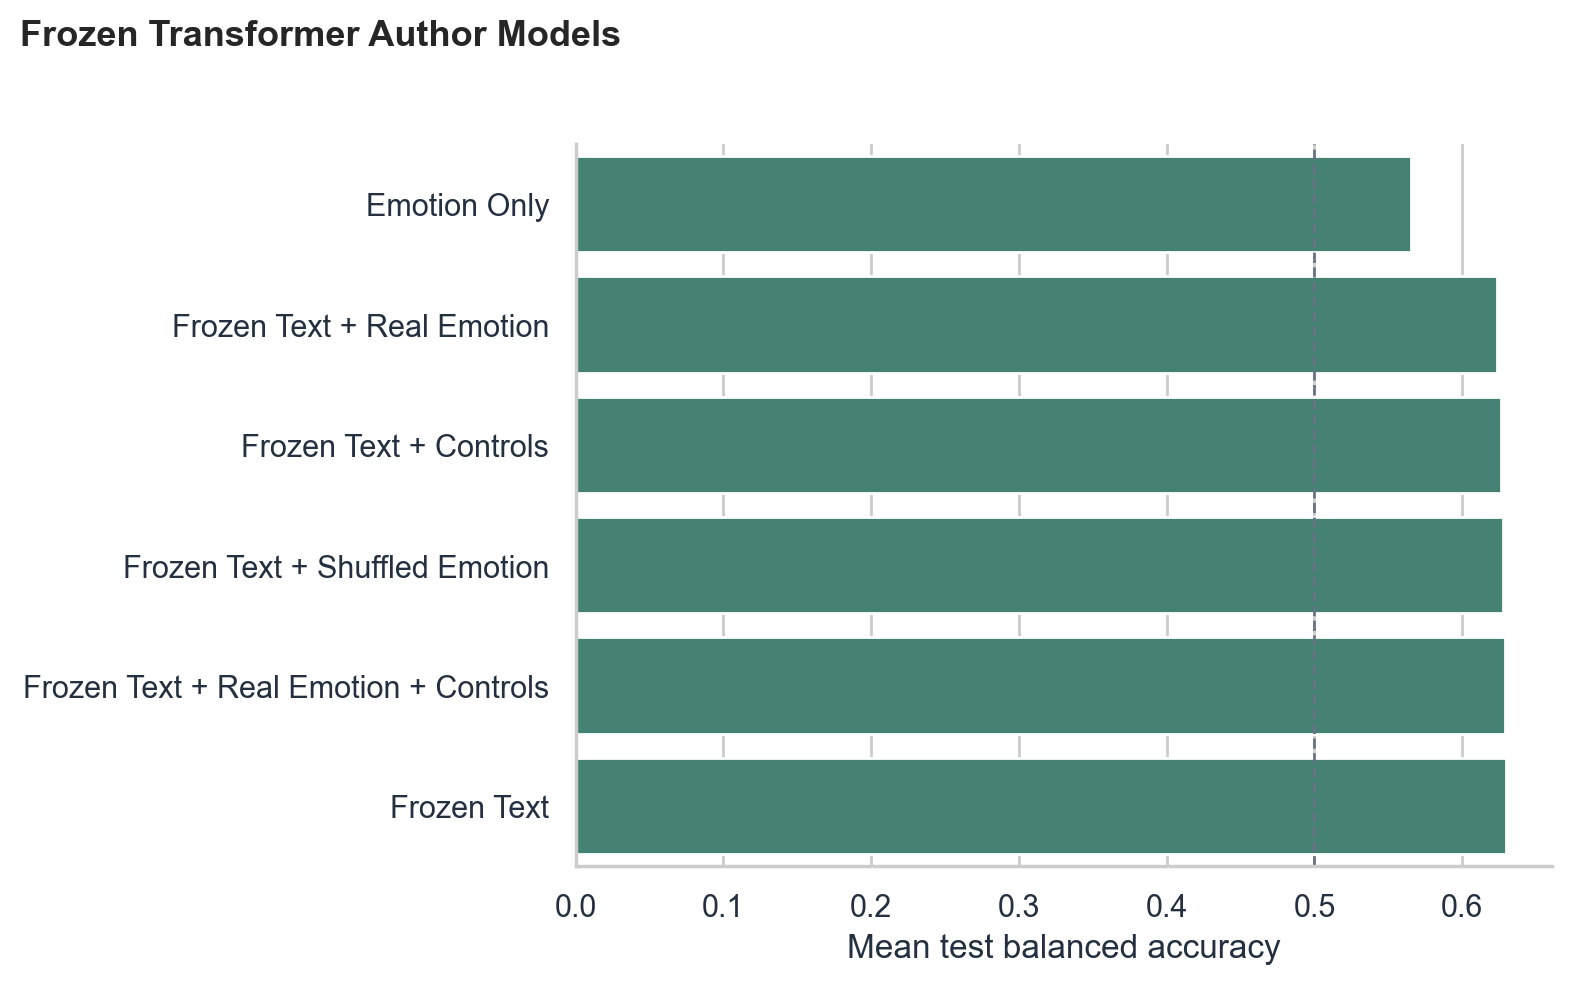
\includegraphics[width=0.78\linewidth]{fig_frozen_transformer_author_models.png}
  \caption{Frozen MiniLM author-probe family. The text + controls and text + real-emotion + controls variants are within $0.001$ of frozen text alone, again consistent with emotion not adding incremental signal under simple pooling.}
\end{figure}

\subsection{Pipeline diagram}

\begin{figure}[H]
  \centering
  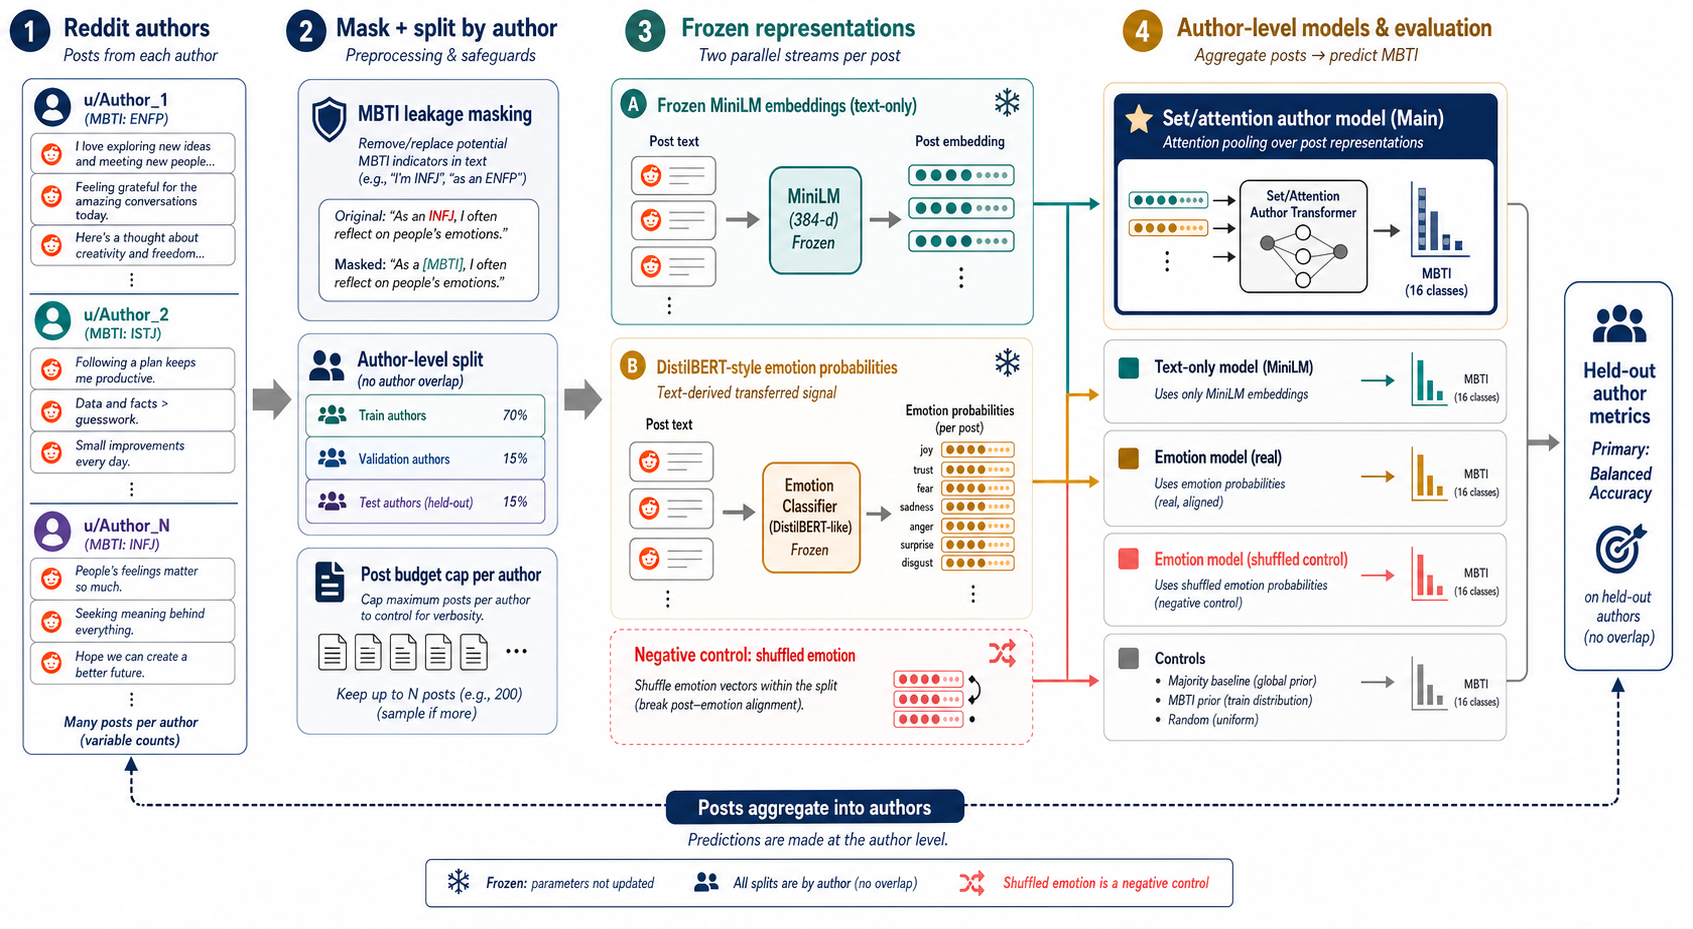
\includegraphics[width=0.95\linewidth]{fig_ms4_pipeline_diagram.png}
  \caption{End-to-end MS4 pipeline. Reddit posts are loaded via KaggleHub, masked for MBTI tokens, filtered, and split by author. Frozen MiniLM produces per-post embeddings; a separate Stage-1 emotion classifier produces transferred emotion probabilities. Author features feed into the baseline layer, the frozen probes, and the set-attention author transformer.}
\end{figure}

\end{document}
